\chapter{Execução do estudo de caso}
\label{cap_estudo_caso_execucao}

Neste capítulo descreveremos como as etapas do estudo de caso foram executadas. Serão fornecidos detalhes a respeito das técnicas utilizadas e como elas foram implementadas no GitResearch.  Por fim, forneceremos os resultados obtidos.

\section{Introdução}

Grande parte das atividades do estudo de caso pôde ser realizada automaticamente. Quando alguma atividade não puder ser automatizada, haverá uma indicação explícita disso. Essa preocupação em automatizar as atividades e documentá-las de forma detalhada foi tomada com o objetivo de permitir que os resultados obtidos no estudo de caso possam ser mais facilmente reproduzidos e reavaliados. 



\section{Seleção}
\label{secao_cap_estudo_selecao_projetos}


  \begin{figure}[H]
  \centering
  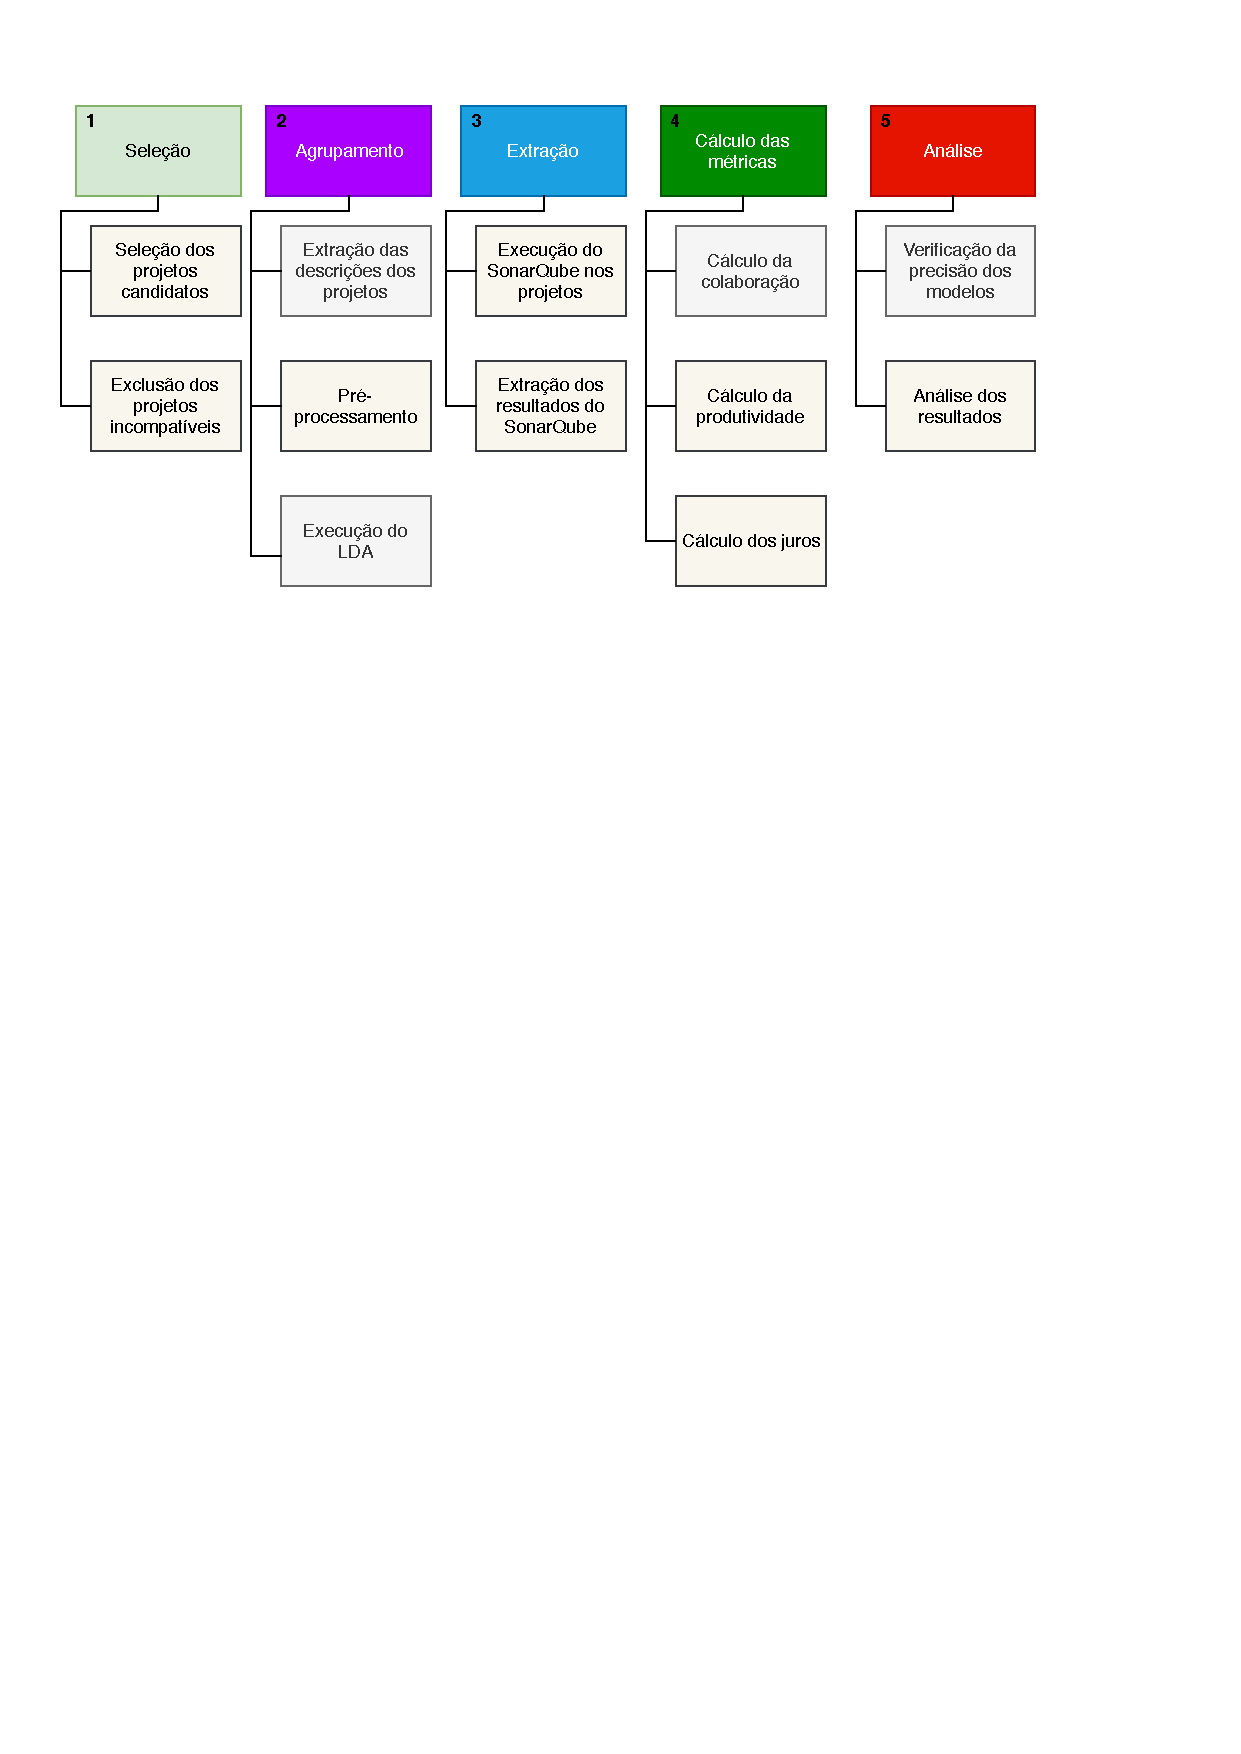
\includegraphics[trim={0.4cm 19.5cm 0cm 1cm},clip]{capitulo_metodo/ResumoEtapas.pdf} 
  \caption{Resumo das etapas do estudo de caso. }
  \label{fig:cap_metodo_resumo_etapas_selecao} 
\end{figure}

\section{Seleção dos projetos candidatos}

Inicialmente, foram selecionados todos os repositórios encontrados no GitHub no momento da execução do estudo de caso.  Essa seleção foi realizada manualmente no GHTorrent  e trouxe como resultado 72.433.097  repositórios. 

\subsection{Exclusão dos projetos incompatíveis}


A seleção dos projetos a serem incluídos neste estudo de caso foi realizada utilizando um conjunto de regras de exclusão. Ou seja, inicialmente selecionamos todos os projetos armazenados no GitHub e depois essas regras de exclusão foram aplicadas fazendo com que o número de projetos diminuísse. Essa estratégia foi usada porque nosso objetivo era incluir a maior quantidade de projetos possível e com isso diminuir a possibilidade de criação de algum viés caso fossem selecionados projetos específicos. Acreditamos que, com isso, a amostra de projetos selecionados é uma representação estatisticamente relevante da população de projetos existentes no GitHub.  As regras de exclusão foram definidas observando três grupos de aspectos da pesquisa:

\begin{enumerate}
\item \textbf{Restrições metodológicas.} Esse grupo de regras inclui aquelas criadas pela necessidade de excluir alguns projetos por eles não possuírem alguma característica obrigatória para a aplicação de algum aspecto da metodologia definida para a pesquisa. Um exemplo é a exclusão de projetos nos quais a descrição não estava na língua inglesa. Essa regra foi criada porque a análise de projetos em múltiplas línguas não é compatível com a atividade de agrupamento de projetos semelhantes. Para essa atividade utilizamos uma técnica de processamento de linguagem natural chamada LDA. Essa técnica agrupa as descrições dos projetos utilizando como base o número de ocorrência de palavras. Se, por exemplo, uma descrição contém diversas vezes as palavras \textit{management} e \textit{database}, o LDA irá criar um tópico com essas duas palavras e inserir nele todos os projetos que possuem também muitas ocorrências dessas duas palavras. Provavelmente, os projetos incluídos serão gerenciadores de banco de dados ou projetos relacionados. Entretanto, caso sejam incluídos projetos de gerenciadores de banco de dados no qual a descrição esteja em outro idioma, e as palavras \textit{management} e \textit{database} fossem escritas nesse idioma, esses projetos poderiam ser colocados em outro tópico. Ou seja, projetos de um mesmo domínio seriam agrupados em grupos diferentes apenas por causa da diferença no idioma da descrição. Por essa razão, foi criada uma regra que removeu todos os projetos que não estavam com a descrição em inglês. Foi escolhido o idioma inglês, pois aproximadamente 70\% dos projetos no GitHub estavam documentados em inglês.
\item \textbf{Restrições operacionais.} Nesse grupo de regras estão aquelas que foram criadas devido a limitações operacionais durante a realização do estudo de caso. Essas restrições, na maior parte das vezes, foram encontradas nas ferramentas utilizadas em algumas etapas da pesquisa. Um exemplo é a ocorrência de falhas durante  a extração das métricas do código-fonte utilizando a ferramenta SonarQube. Alguns projetos não puderam ter seu código-fonte analisado por essa ferramenta mesmo após diversas tentativas e o acionamento do suporte da ferramenta. Com isso, esses projetos tiveram de ser excluídos já que uma extração manual dessa métricas era inviável devido ao tamanho dos projetos. Ainda nesse grupo de regras de exclusão estão aquelas que foram criadas devido à incompatibilidade com o sistema operacional utilizado. Alguns arquivos tinham nomes muito extensos ou utilizavam caracteres que não eram aceitos pelo sistema operacional que foi utilizado para a execução do estudo de caso. Isso levou à exclusão dos projetos que continham os arquivos que geraram esses problemas.
\item \textbf{Inclusão apenas de repositórios de software. } O último grupo de regras é formado por aquelas que foram criadas para excluir repositórios que não sejam projetos de desenvolvimento de software. Conforme já mencionado no item \ref{cap_estudo_github}, muitos dos repositórios criados no GitHub são usados apenas para armazenar arquivos. Para excluir esses repositórios, nós utilizamos regras sugeridas pela literatura. Além disso, após a realização de análises preliminares da lista de projetos, também criamos nossas regras de exclusão. Com isso, um número substancial de repositórios foi removido da pesquisa. 
\end{enumerate}

A Tabela \ref{table:regras_exclusao} contém uma lista com todas as regras de exclusão utilizadas para a seleção dos projetos. As regras estão ordenadas na tabela na ordem em que foram aplicadas. Nessa tabela fornecemos uma descrição da regra, indicamos se ela se trata de uma regra metodológica, operacional ou para verificar se o repositório é realmente um projeto de software. Além disso, informamos se a regra foi aplicada utilizando como base os dados no GHTorrent ou houve a necessidade de acessar o código-fonte do projeto.  Por fim, informamos a quantidade de projetos que foram removidos por cada regra de exclusão. 


\def\arraystretch{2.5}
\begin{longtable}{|c|c|c|c|c|}

\hline
\# & \pbox{8cm}{Descrição}                                                                            & Tipo     & Local     & \pbox{1.7cm}{Projetos Excluídos} \\ \hline
1  & \pbox{8cm}{Exclusão de projetos abandonados, exemplos, exercícios, tutoriais e projetos android.} & Software & GHTorrent &     20.512.447\\ \hline
2  & \pbox{8cm}{Exclusão de projetos que não utilizem a linguagem de programação Java.} & Metodológica & GHTorrent &    48.385.193       \\ \hline
3  & \pbox{8cm}{Exclusão de projetos deletados.} & Software & GHTorrent &    367.570       \\ \hline
4  & \pbox{8cm}{Exclusão de projetos que são \textit{Forks} de outros projetos.} & Metodológica & GHTorrent &    1.637.704       \\ \hline
5  & \pbox{8cm}{Exclusão de projetos sem descrição no GHTorrent.} & Metodológica & GHTorrent &     595.557      \\ \hline
6  & \pbox{8cm}{Exclusão de projetos no qual a descrição não esteja em inglês.} & Metodológica & Código-fonte &     342.925      \\ \hline
7  & \pbox{8cm}{Exclusão de projetos que tenham poucos \textit{commits} e poucos colaboradores.} & Software & GHTorrent &    588.909       \\ \hline
8  & \pbox{8cm}{Exclusão de projetos com nomes de arquivos incompatíveis.} & Operacional & Código-fonte &  126         \\ \hline
9  & \pbox{8cm}{Exclusão de projetos nos quais o SonarQube não foi capaz de analisar o código.} & Operacional & Código-fonte &      54     \\ \hline
10  & \pbox{8cm}{Exclusão de projetos com arquivo de descrição inexistente ou muito pequeno .} & Metodológica & Código-fonte &   726        \\ \hline
11 & \pbox{8cm}{Exclusão de projetos muito grandes .} & Operacional & Código-fonte &      72     \\ \hline

\caption{Regras para a exclusão de projetos do estudo de caso}
\label{table:regras_exclusao}
\end{longtable}
\def\arraystretch{1}


É necessário detalhar a motivação de algumas das regras de exclusão criadas:

\begin{itemize}
\item[\textbf{Regra 2}] Remove projetos que não foram realizados utilizando a linguagem Java. Essa regra foi definida por dois motivos. O primeiro motivo é a diferença que existe entre as dívidas técnicas de uma linguagem e outra. Por exemplo, existem dívidas específicas para linguagens orientadas a objetos que não são possível de serem encontradas em linguagens procedurais. O segundo motivo é técnico e está relacionado com as limitações da ferramenta utilizada para a extração de métricas. Ela possui uma maior compatibilidade com a linguagem Java.
\item[\textbf{Regra 4}] Evita que projetos duplicados sejam incluídos na pesquisa. No GitHub, um \textit{Fork} é um procedimento onde um usuário realiza uma cópia, para a sua conta, de um repositório \cite{thung2013network}. Esse procedimento é realizado quando esse usuário deseja contribuir com esse repositório original ou quando ele tem interesse em iniciar um novo projeto tendo como base esse repositório inicial. Em ambos os casos, esses dois repositórios serão muito parecidos. Logo, resolvemos remover esses repositórios que foram gerados por meio de um \textit{Fork}.
\item[\textbf{Regra 6}] Exclui projetos nos quais a documentação não está escrita em inglês. O motivo dessa restrição foi a necessidade de separar os projetos por domínio de aplicação. Essa separação foi feita aplicando técnicas de aprendizado de máquina  na documentação dos projetos.  A inclusão de múltiplas linguagens iria trazer uma complexidade substancial a esse processo. Além disso, a técnica de classificação que será utilizada não é compatível com textos em múltiplas linguagens.
\item[\textbf{Regra 7}] Remove os projetos que tinham menos de 6 colaboradores e um número de \textit{commits} menor do que 516. Essa exclusão foi realizada com o objetivo de remover da pesquisa os repositórios que não são projetos de software. De acordo com Bird et al.\cite{bird2009promises}, o número de colaboradores e o número de \textit{commits} são uma forma eficaz de identificar repositórios que tenham sido criados apenas para a realização de testes, que sejam exemplos de código ou que sejam projetos particulares. De acordo com os autores,  se um repositório teve uma quantidade mínima de \textit{commits} e colaboradores, há uma probabilidade maior de que seja um projeto de software real. Os números mínimos utilizados nesta pesquisa foram obtidos por meio de análises dos projetos existentes no GitHub. Foi encontrada uma média desses números em todo o conjunto de projetos do GitHub e a essa média foi adicionada uma margem de dois desvios padrão. 
\item[\textbf{Regra 11}] Excluir projetos com uma quantidade muito grande de arquivos. Essa regra foi criada por dois motivos. O primeiro foi a impossibilidade de o SonarQube processar alguns desses projetos. Mesmo após diversas tentativas e o acionamento do suporte da ferramenta, não pudemos processá-los. O segundo motivo é a observação de que repositórios com muitos arquivos normalmente não são projetos de software. em vez disso, eles são criados para armazenar logs e outros tipos de arquivos que não têm relação com o desenvolvimento de software.
\end{itemize} 



Algumas das regras encontradas na Tabela  \ref{table:regras_exclusao} foram criadas para excluir repositórios que não são projetos de software. Na literatura podemos encontrar algumas recomendações práticas de como evitar problemas na utilização de dados do GitHub em pesquisas científicas \cite{kalliamvakou2014promises,bird2009promises,tsay2014influence}.  Algumas das recomendações que foram consideradas na criação das regras de exclusão foram:

\begin{itemize}
\item \textbf{Nem sempre um repositório no GitHub é utilizado para armazenar um projeto de software.} Apesar de ser voltado para a hospedagem de projetos de software, o GitHub não impõe nenhum tipo de restrição ao conteúdo dos repositórios que ele armazena. Por ser uma plataforma gratuita, isso faz com que muitos usuários o utilizem para o armazenamento de arquivos diversos.  É comum encontrar arquivos de sites, exercícios escolares, contratos e diversos outros itens que não têm relação com o objeto desta pesquisa. Para evitar a inclusão de repositórios que não armazenam projetos de software, utilizamos uma série de heurísticas, algumas delas sugeridas por Killiamvakou et al.\cite{kalliamvakou2014promises} e outras criadas especificamente para esta pesquisa. 
\item \textbf{Muitos projetos não são totalmente desenvolvidos no GitHub.} Esses desenvolvimentos fora do GitHub pode ser de duas formas: prévio e paralelo. Um projeto pode ser desenvolvido previamente em uma outra plataforma e depois ser migrado para o GitHub. Essa migração pode ser feita importando todo o histórico do projeto como também, esse histórico pode ser ignorado. Isso precisa ser considerado já que nesses casos esse histórico anterior pode ser relevante para a pesquisa sendo realizada.  A outra forma de desenvolvimento fora do GitHub é quando algumas das atividades necessárias para o desenvolvimento do projeto não são realizadas no GitHub ou são realizadas parcialmente. Um exemplo seria o gerenciamento de \textit{issues} que pode ser feito no GitHub ou em outro serviço como o FindBugs\cite{ayewah2007using}. Assim, uma pesquisa poderia, equivocadamente, realizar conclusões com base em dados incompletos. O caso em que poderia haver algum impacto nos resultados desta pesquisa é o de desenvolvimento prévio. Caso um projeto fosse criado no GitHub sem que o histórico fosse importando, nossas análises de produtividade não poderiam ser feitas utilizando essa contribuição prévia. Para evitar esse problema, utilizamos, novamente, um conjunto de heurísticas baseadas nas datas de criação dos arquivos do repositório e nas datas dos primeiros \textit{commits} realizados no GitHub. Se um repositório possuía um arquivo com uma data muito anterior ao primeiro \textit{commit}, esse repositório provavelmente teve um desenvolvimento prévio fora do GitHub e, portanto, deveria ser excluído da pesquisa.
\end{itemize}





No banco de dados do GHTorrent há um total de 72.433.097 repositórios. Após a aplicação das onze regras de exclusão listadas na Tabela \ref{table:regras_exclusao}, sobrou um total de 1.814 repositórios.  Dessa forma, neste estudo de caso analisaremos 1.814 repositórios de software.

\section{Agrupamento dos projetos}

  \begin{figure}[H]
  \centering
  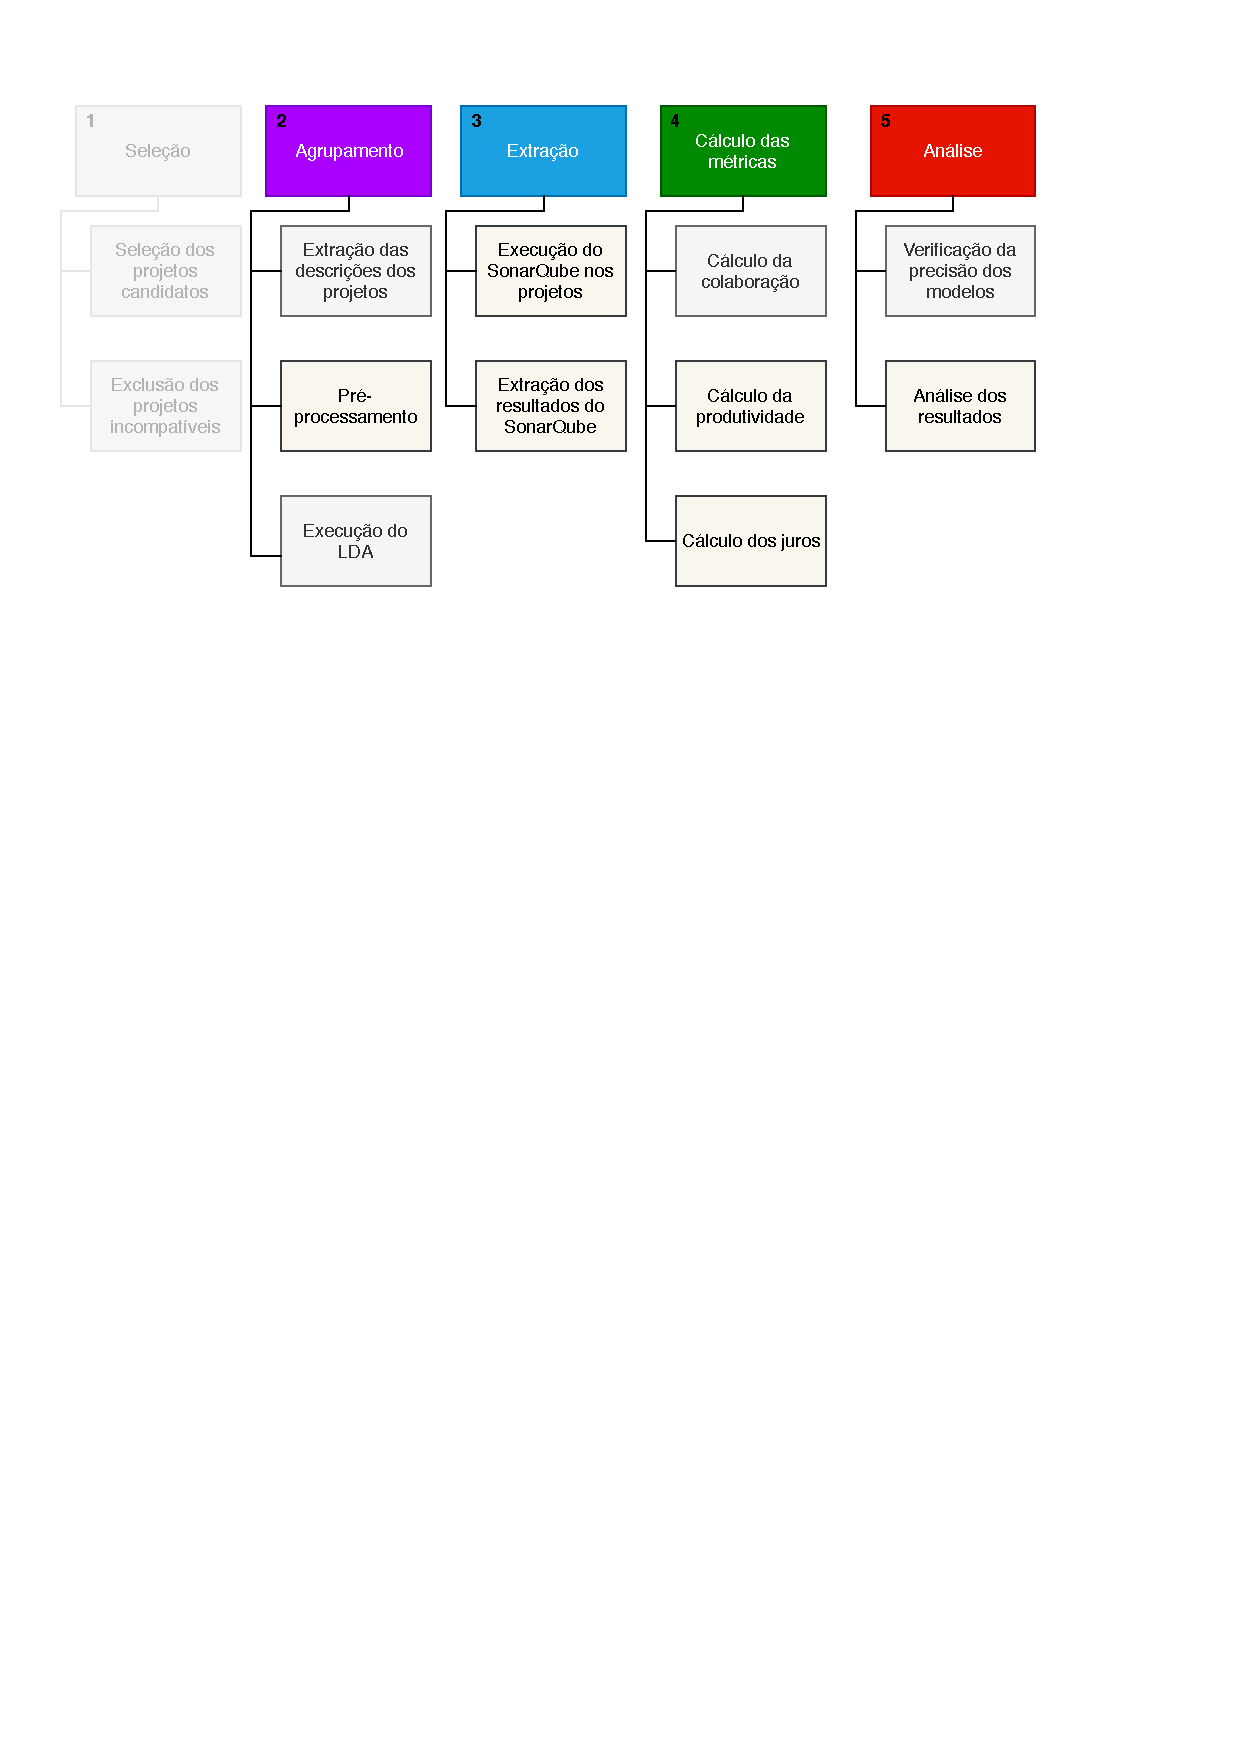
\includegraphics[trim={0.4cm 19.5cm 0cm 1cm},clip]{capitulo_estudo_caso/EtapasAgrupamento.pdf} 
  \caption{Resumo das etapas do estudo de caso. }
  \label{fig:cap_metodo_resumo_etapas_agrupamento} 
\end{figure}


De acordo com Kitchenham et. al.\cite{kitchenham2004software}, a comparação de produtividade entre projetos de software deve ser feita considerando o domínio de cada um deles. Portanto, não faz sentido comparar a produtividade de um projeto da área da aviação, que possui padrões extremamente rígidos de qualidade, com um projeto de uma aplicação para a internet. Por isso, os projetos utilizados no estudo de caso foram divididos em domínios de aplicação como sistemas gerenciadores de banco de dados, jogos, frameworks, linguagens de programação, etc.

Inicialmente foram consideradas algumas estratégias para estimação do domíno do projeto. Uma delas foi a proposta de Idri. et. al.\cite{idri2001fuzzy}. Nela, os autores utilizam um modelo baseado em lógica Fuzzy para estimar o domínio de um projeto de software. Além disso, foram estudas outras abordagens baseadas no código fonte da aplicação. Entre elas estão o trabalho de Yamamoto et. al.\cite{yamamoto2005measuring} e a ferramenta MudaBlue, proposta por Kawaguchi et. al.\cite{kawaguchi2006mudablue}. Essas abordagens não foram utilizadas já que dependiam de informações a que não tínhamos acesso ou da construção do projeto. Como utilizamos uma abordagem automática, muitas vezes não era possível compilar os projetos devido a algum erro no código, incompatibilidade com o ambiente ou falta de alguma dependência. 

Nosso modelo de estimação dos juros da Dívida técnica é baseado na comparação das produtividades de projetos que possuam pouca dívida técnica e projetos que possuem um nível médio ou alto da dívida técnica. Entretanto, essa comparação será feita apenas entre projetos de um mesmo domínio de aplicação. Por exemplo, arcabouços de desenvolvimento como o Spring Batch\cite{cogoluegnes2011spring}, que foi usado para desenvolver a ferramenta GitResearch, só terá sua produtividade comparada com outros projetos que também sejam arcabouços de desenvolvimento ou estejam relacionados a arcabouços de desenvolvimento.  Neste estudo de caso, realizaremos esse agrupamento dos projetos por domínio utilizando uma técnica de processamento de linguagem natural chamada \textit{Latent Dirichlet Allocation}( LDA). Extrairemos de cada projeto a sua descrição e aplicaremos o LDA para identificar o seu domínio.

\subsection{Extração das descrições dos projetos}

Para a execução do LDA foi necessário extrair a descrição de cada projeto. Essa descrição foi obtida do próprio repositório onde o projeto é armazenado. Esse procedimento pôde ser feito já que há uma padronização em relação ao nome do arquivo onde a descrição do projeto deve ser inserida. Esse arquivo fica localizado no diretório raiz do repositório e normalmente recebe o nome de \textit{readme.md}. Entretanto, é possível que sejam usadas variações desse nome como \textit{readme.txt} e \textit{readme.html}. Quando nem  o arquivo padrão nem  alguma das variações foram encontradas, foi utilizado qualquer arquivo no qual o nome inicia com a palavra readme. Se mesmo assim, não foi encontrado nenhum arquivo, então o projeto foi excluído da pesquisa conforme a regra 10 da Tabela \ref{table:regras_exclusao}.

\subsection{Pré-processamento}

Após a extração da descrição de cada projeto, foi necessário realizar uma série de manipulações textuais nas descrições de tal  forma que  elas pudessem ser utilizadas com o LDA. Essas manipulações incluem a remoção de palavras irrelevantes como preposições e artigos, remoção de marcações HTML e XML, a remoção de caracteres especiais e a redução de palavras para sua forma comum(\textit{stemming}\cite{jivani2011comparative}).  Essas modificações foram realizada no GitResearch por meio da classe \textit{DescriptionNormalizer}. Cada uma das transformações foi escrita em uma classe individual e inseridas no grupo padrão de transformações. Em outras pesquisas, será possível criar novos grupos de transformações.  A Tabela \ref{table:transformacoes_lda} apresenta uma lista com todas as classes de transformação que foram utilizadas no pré-processamento das descrições.


\begin{table}[H]

\def\arraystretch{2.5}
\begin{tabular}{|c|c|}

\hline
\textbf{Classe}                                 & \pbox{8cm}{\textbf{Transformação}}                                                                            \\ \hline
RemoveUrlTransformation                & \pbox{8cm}{Remove todas as URL do texto }                                                            \\ \hline
RemoveXmlTransformation                & \pbox{8cm}{Remove todas as marcações HTML e XML}                                                     \\ \hline
RemoveEspecialCharactersTransformation & \pbox{8cm}{Remove caracteres especiais}                                                              \\ \hline
RemoveSpacesTransformation             & \pbox{8cm}{Remove espaços múltiplos}                                                                 \\ \hline
RemoveNumbersTransformation            & \pbox{8cm}{Remove todos os números}                                                                  \\ \hline
LowerCaseTransformation                & \pbox{8cm}{Transforma todo o texto em minúsculo}                                                    \\ \hline
RemoveStopWordsTransformation          & \pbox{8cm}{Remove palavras como "the" e "and" que são irrelevantes  para a categorização dos textos} \\ \hline
RemoveLicenseWordsTransformation       & \pbox{8cm}{Remove texto a respeito das licenças dos softwares}                                      \\ \hline
\end{tabular}
\def\arraystretch{1}
\caption{Transformações realizadas no texto das descrições dos projetos}
\label{table:transformacoes_lda}
\end{table}


\subsection{Execução do LDA}

O LDA considera que um documento é formado por palavras que, por sua vez, estão relacionadas a um tópico.  As palavras são associadas a um tópico automaticamente durante a análise do conjunto de documentos. Se uma palavra $w_1$ aparece em muitos documentos junto com uma palavra $w_2$, o LDA assume que há uma relação semântica entre essas palavras e por isso elas devem ficar em um mesmo tópico. Um exemplo seriam as palavras \textit{player}, \textit{game} e \textit{joystick}. Essas palavras normalmente seriam muito encontradas nas descrições dos projetos relacionados aos jogos eletrônicos. Isso faria com o LDA criasse um tópico com essas e outras palavras relacionadas aos jogos e associasse esse tópico a todos os documentos nos quais elas aparecem muitas vezes. 

O LDA baseia-se na ideia de que cada documento analisado foi gerado por uma combinação de  X\% de palavras de um tópico $A$, Y\% de um tópico $B$ e assim por diante. Sendo assim, dado um documento $D$, o LDA realiza o caminho inverso  para identificar o quanto do tópico $A$ foi usado para gerar o documento $D$, o quanto do tópico $B$ foi usado para gerar o documento $D$ e assim por diante. 


A execução do LDA foi realizada da seguinte forma:

\begin{enumerate}
\item Foi definido o número de tópicos que serão utilizados. É importante notar que o LDA exige apenas a quantidade e não quais são esses tópicos. Neste estudo de caso, utilizamos o número 30. Esse número foi escolhido após a realização de experimentos no qual vários números foram testados. Com uma quantidade muito grande de tópicos percebemos que alguns deles ficaram com apenas um ou nenhum projeto. Quando um número muito pequeno de tópicos foi escolhido, percebemos que alguns dos tópicos gerados claramente misturavam mais de um assunto. Além disso, o número 30 foi escolhido por ser um número próximo do utilizado em outros trabalhos semelhantes como o de Ray et al.\cite{ray2014large}. 
\item O algoritmo foi aplicado no conjunto de arquivos de descrição dos projetos. No primeiro momento ele descobre quais palavras pertencem a cada um dos 30 tópicos. Isso é feito ao identificar quais palavras normalmente aparecem juntas nos documentos.
\item A quantidade de palavras de cada tópico em cada documento irá  definir o quanto aquele documento é sobre aquela categoria. O tópico com mais palavras dentro do documento é considerado o seu tópico principal.
\end{enumerate}









\subsubsection{Resultado do LDA}

A Tabela \ref{table:topicos_lda} apresenta todos os 30 tópicos e suas respectivas palavras. Conforme pode ser visto, as palavras estão em sua forma reduzida devido à aplicação do \textit{stemming}. Um exemplo pode ser visto no Tópico 12. A primeira palavra desse tópico é a palavra ``test''. Entretanto, na verdade, essa palavra representa todas as palavras que contêm o prefixo ``test'', como ``testing'', ``tests'', ``testability'' e assim por diante. 

É importante destacar que as palavras estão sendo exibidas na tabela \ref{table:topicos_lda} ordenadas pelo seu nível de relevância dentro do tópico. Por isso, para identificar qual domínio cada tópico representa, a primeira palavra deve ser a mais decisiva.  Existem alguns tópicos nos quais as suas palavras permitem-nos claramente identificar o domínio que ele representa. Esse é o caso do tópico 22 que agrupará os projetos relacionados aos jogos eletrônicos. Outro exemplo é o Tópico 23 que agrupará projetos relacionados ao processamento distribuído de dados. Enquanto isso, alguns tópicos não nos permitem identificar qual domínio eles representam. 



\def\arraystretch{2.5}
\begin{longtable}{|c|c|}
\hline
\textbf{Nome} & \pbox{13cm}{\textbf{Palavras}}                                                                                                                                             \\ \hline
Tópico 1          & \pbox{13cm}{applic android fix xprivacy addon restrict support ad data devic forg app play improv processor return permiss mode googl map }                       \\ \hline
Tópico 2          & \pbox{13cm}{index elasticsearch cassandra data set search json type file query solr field document fs true default test map bin support}                          \\ \hline
Tópico 3          &\pbox{13cm}{ build instal java run file jar directory packag ant sourc command window download compil path test linux document git bin }                           \\ \hline
Tópico 4          &\pbox{13cm}{ connect client server user authent command default host session key configur ssh option password set login request winrm overther file}               \\ \hline
Tópico 5          &\pbox{13cm}{ query api custom item id storefront checkout respons field widget java chart content overrid v1 terasoluna type gfw public payment }                  \\ \hline
Tópico 6          & \pbox{13cm}{distribut export wicket includ govern inform encrypt law file h2o security requir build impli kind cryptograph applic country import condit}          \\ \hline
Tópico 7          &\pbox{13cm}{ docker servic run imag doc user contain cluster api creat meso aw compos configur karaf url command provid build jame}                                \\ \hline
Tópico 8          & \pbox{13cm}{stream sampl data event file configur messag parser log queue tnt4j activ xml defin field property string chronicl paramet entri}                     \\ \hline
Tópico 9          & \pbox{13cm}{applic develop servic manag web support data base system server framework user compon model build platform api integr document modul}                 \\ \hline
Tópico 10         & \pbox{13cm}{java report attribut set job user operationresult resourc servic row session method id column client jasperadmin organ request list server}           \\ \hline
Tópico 11         & \pbox{13cm}{java class method public string type return annot builder final object map static xml gener interfac org api void person}                             \\ \hline
Tópico 12         & \pbox{13cm}{test driver tabl databas java run jdbc engin configur execut gwt sql default requir assert selenium junit user connect firefox}                       \\ \hline
Tópico 13         &\pbox{13cm}{ issu contribut build develop sourc document code statu support list maven download badg open bug request mail doc api wiki}                           \\ \hline
Tópico 14         & \pbox{13cm}{java core imag question demo src main aima text link student answer ui search org jar library post bridgedb afc}                                      \\ \hline
Tópico 15         & \pbox{13cm}{graph java data algorithm handlebar src script templat workflow input comment structur output languag code taverna jwetherel compil task yesworkflow} \\ \hline
Tópico 16         & \pbox{13cm}{file library format imag jar support data gnu gener includ sourc java public code free distribut form common term work}                               \\ \hline
Tópico 17         &\pbox{13cm}{ click sdk select modul file elixir function tab run png screenshot button line true configur menu test open view raw}                                 \\ \hline
Tópico 18         & \pbox{13cm}{matrix de jsf msf4j openbaton implement jersey opengl microservic chouett redisson build matrix4f baton microserv joml transform en dddlib ob1k }     \\ \hline
Tópico 19         & \pbox{13cm}{test simul run remot worker coordin hazelcast start client command agent machin member predict file benchmark cflint java script map}                 \\ \hline
Tópico 20         & \pbox{13cm}{file set code support option creat time number work make note provid class chang type default configur user system includ}                            \\ \hline
Tópico 21         &\pbox{13cm}{ run server databas instal test configur applic file build start deploy properti tomcat mysql user mvn default web db war}                             \\ \hline
Tópico 22         &\pbox{13cm}{ game mod player minecraft team robot openmr block server main make item build play develop creat place piec gener asset}                              \\ \hline
Tópico 23         &\pbox{13cm}{ build eclips plugin run test maven instal mvn gradl jar gradlew repository java file modul command id target clean org}                               \\ \hline
Tópico 24         & \pbox{13cm}{data model research analysi databas tool develop rif univers genom gener base public peptideshak comput health repository inform sourc design}        \\ \hline
Tópico 25         & \pbox{13cm}{data hadoop spark cluster distribut index node oper read random algorithm process scala exampl deep learn model machin comput pipelin}                \\ \hline
Tópico 26         & \pbox{13cm}{api modul schema swagger uri file gener json java document config client batch data library marklog corb javascript codegen option}                   \\ \hline
Tópico 27         &\pbox{13cm}{ spring cloud googl java client code repository applic data servic maven io boot id build add core info pull sourc}                                    \\ \hline
Tópico 28         &\pbox{13cm}{ cach counter morphium neo4j info mongodb transact id xxx current data main iteratortest java object query public privat string wrong}                 \\ \hline
Tópico 29         & \pbox{13cm}{git master branch build tool repository commit pull yourkit clone server plugin push repo job merg upstream fork request instal}                      \\ \hline
Tópico 30         & \pbox{13cm}{android java studio app event weblog output gem api intern stanford read test statu connect result io ssl relex notif}                                \\ \hline

\caption{Tópicos e suas palavras.}
\label{table:topicos_lda}
\end{longtable}
\def\arraystretch{1}
 
 
 É evidente que nosso agrupamento dos projetos por domínio utilizando apenas sua descrição jamais será totalmente preciso. Isso acontece tanto por imprecisões no LDA quanto por causa do conteúdo das descrições dos projetos. Em alguns casos, essa descrição não permite nem mesmo que um especialista em software consiga identificar qual o propósito do projeto e em qual domínio ele se encaixa. Ainda assim, acreditamos que esse agrupamento aproximado possa ser utilizado de forma eficaz para aumentar a precisão do nosso modelo de estimação dos juros da dívida técnica. De qualquer forma, ao analisarmos os resultados finais do estudo de caso, iremos comparar os dados obtidos quando realizamos o agrupamento por domínio e quando não realizamos esse agrupamento. 



\section{Extração dos dados}

  \begin{figure}[H]
  \centering
  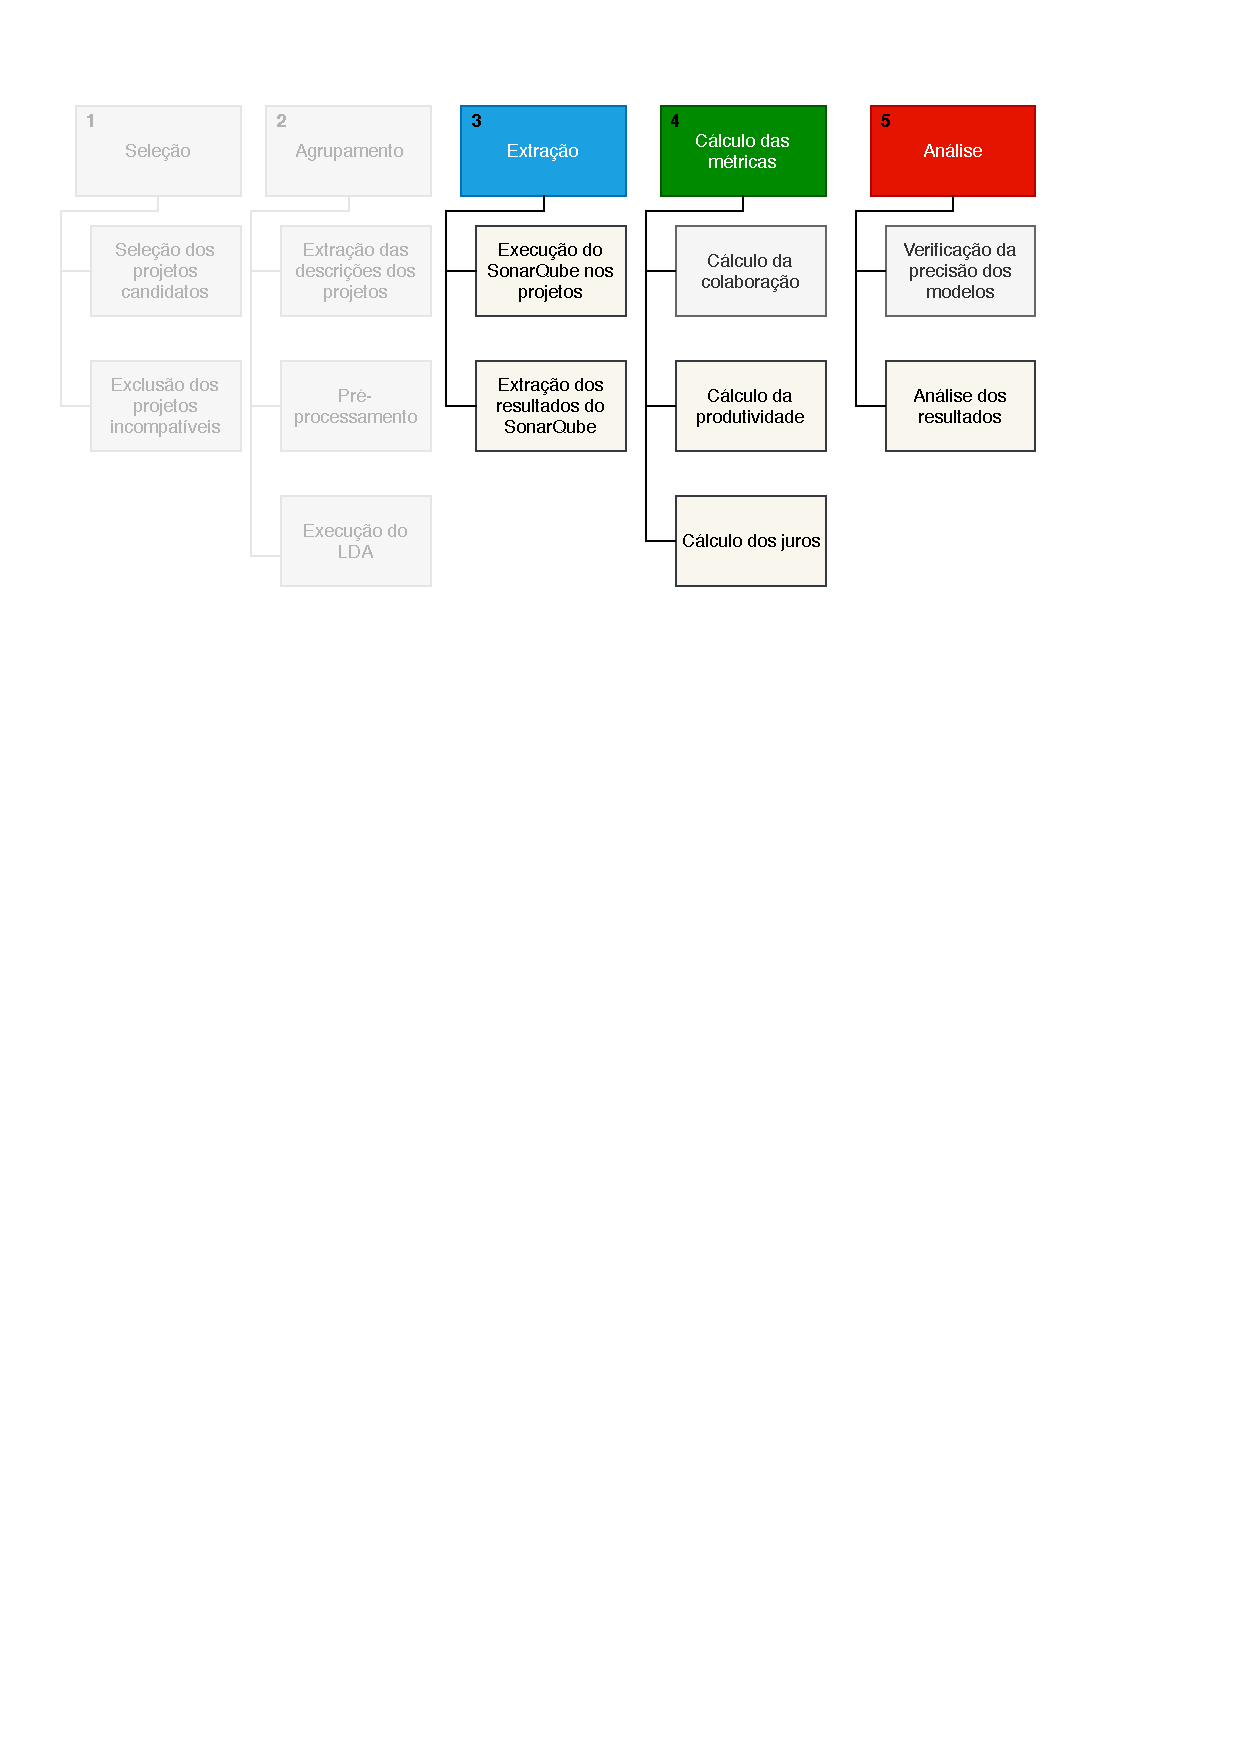
\includegraphics[trim={0.4cm 19.5cm 0cm 1cm},clip]{capitulo_estudo_caso/EtapasExtracao.pdf} 
  \caption{Resumo das etapas do estudo de caso. }
  \label{fig:cap_metodo_resumo_etapas_extracao} 
\end{figure}


Nesta etapa do estudo de caso, iremos extrair os dados dos projetos selecionados. Serão extraídas diversas métricas comumente utilizadas para a avaliação de projetos de software tais como quantidade de arquivos, linhas de código e complexidade. Além disso, nessa etapa iremos medir o nível de dívida técnica de cada um dos projetos.  Tanto as métricas do software quanto a dívida técnica serão medidas utilizando a ferramenta SonarQube\cite{campbell2013sonarqube}. Algumas outras informações como popularidade e colaboração serão obtidas do GHTorrent. 

\section{Execução do SonarQube nos projetos}
 
Todas as métricas obtidas do código-fonte dos projetos foram extraídas em cinco pontos diferentes na evolução do software.  Para realizar essa divisão utilizamos a quantidade de \textit{commits} de cada projeto. Por exemplo, se um projeto tem 1.000 \textit{commits}, fizemos a extração das métricas quando o projeto tinha apenas 200, depois quando tinha 400,600,800 e finalmente 1.000 \textit{commits}.  A Figura \ref{fig:codigo_conta_commits} exibe a porção de código no GitResearch responsável pela contagem dos \textit{commits} de um projeto. É possível notar que não basta apenas contar a quantidade de \textit{commits} já que, como mostrado na Figura \ref{fig:cap_experimento_exemplo_grafo_git_merge}, é possível que um \textit{commit} esteja envolvido em algum \textit{merge} e por isso possua mais de um pai. Para resolver esse problema e podermos navegar corretamente no grafo de \textit{commits}, nós consideramos apenas o primeiro pai encontrado conforme pode ser visto na linha 21 da Figura \ref{fig:cap_experimento_exemplo_grafo_git_merge}. O código responsável por executar o SonarQube em cada projeto é exibido na Figura \ref{fig:codigo_executa_sonar}. Mais detalhes sobre como o Git armazena as versões do software podem ser encontrados no Apêndice \ref{apendice_git}.

 \begin{figure}[H]
  \centering
  \frame{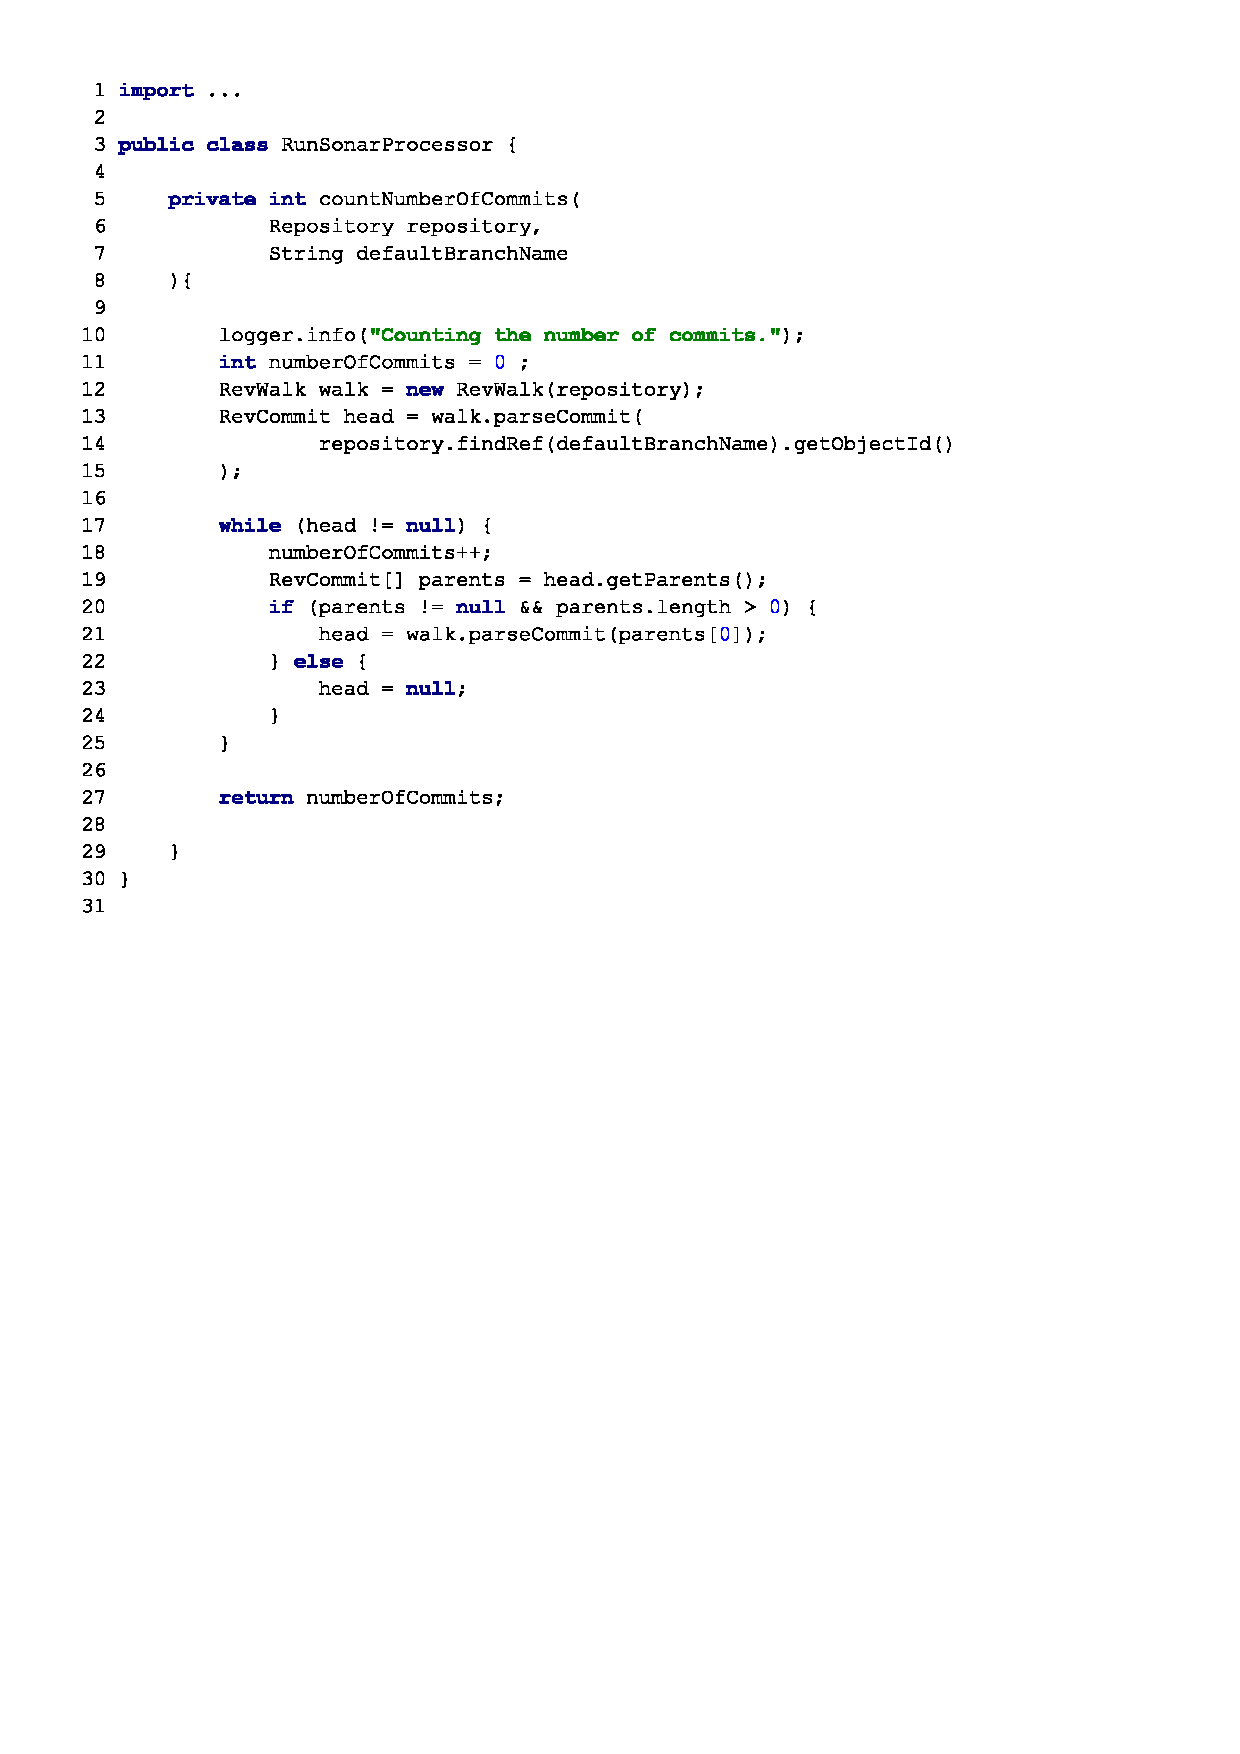
\includegraphics[trim={1cm 14cm 2.5cm 0},clip]{capitulo_estudo_caso/codigo_conta_commits.pdf}} 
  \caption{Código do GitResearch responsável por contar a quantidade de \textit{commits} de cada projeto.}
  \label{fig:codigo_conta_commits} 
\end{figure}

 \begin{figure}[H]
  \centering
  \frame{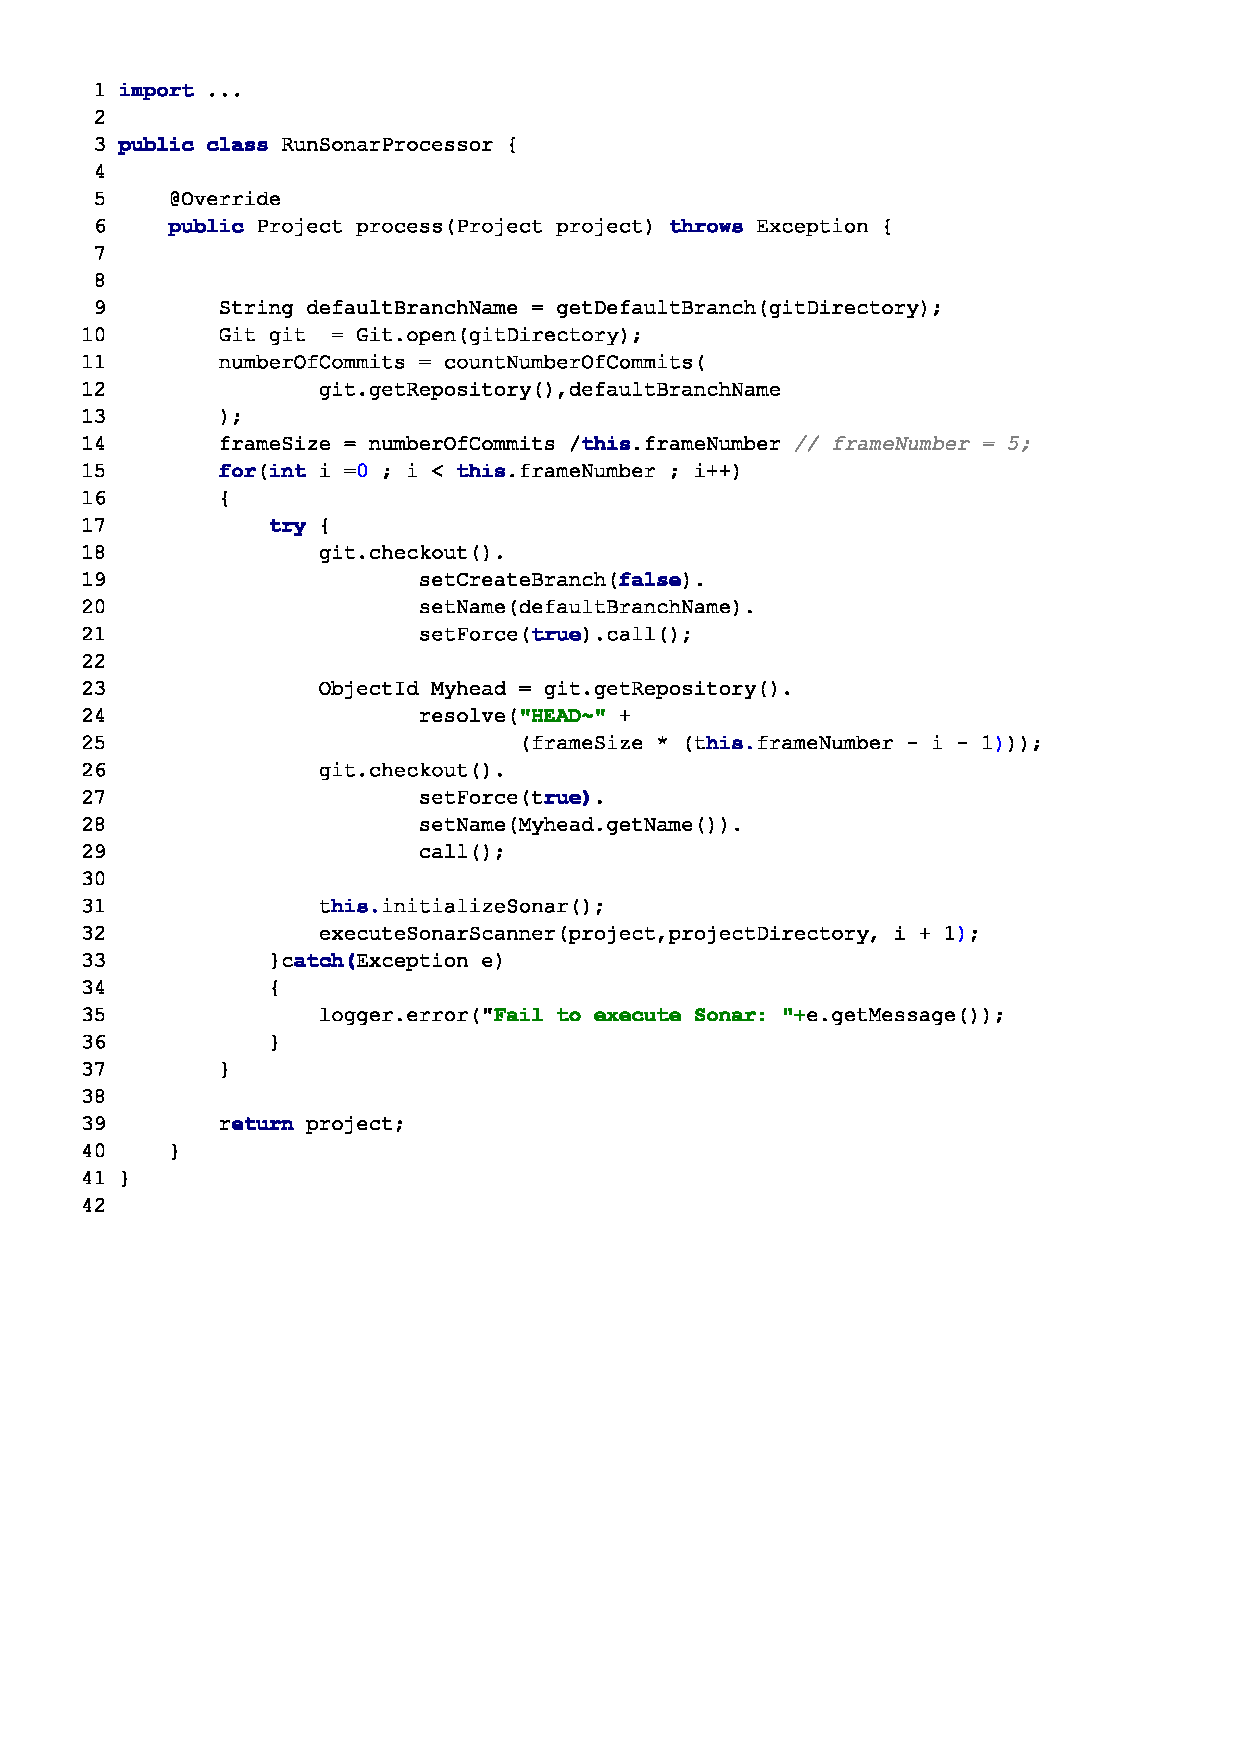
\includegraphics[trim={1cm 9cm 2.5cm 0},clip]{capitulo_estudo_caso/codigo_executa_sonar.pdf}} 
  \caption{Código responsável por executar o \textit{scanner} do SonarQube em cada projeto.}
  \label{fig:codigo_executa_sonar} 
\end{figure}

\section{Extração dos resultado do SonarQube}

Após a execução do SonarQube em todos os projetos do estudo de caso, tivemos que realizar um processo para extrair os dados obtidos e utilizá-los nas demais etapas do estudo de caso. Essa extração foi realizada pelo GitResearch utilizando a API fornecida pelo SonarQube. Todos os dados gerados podem ser obtidos no seguinte link: https://github.com/Jandisson/git-research/raw/master/DADOS\_BRUTOS\_PROJETOS.xlsx.





 


\section{Cálculo das métricas}


  \begin{figure}[H]
  \centering
  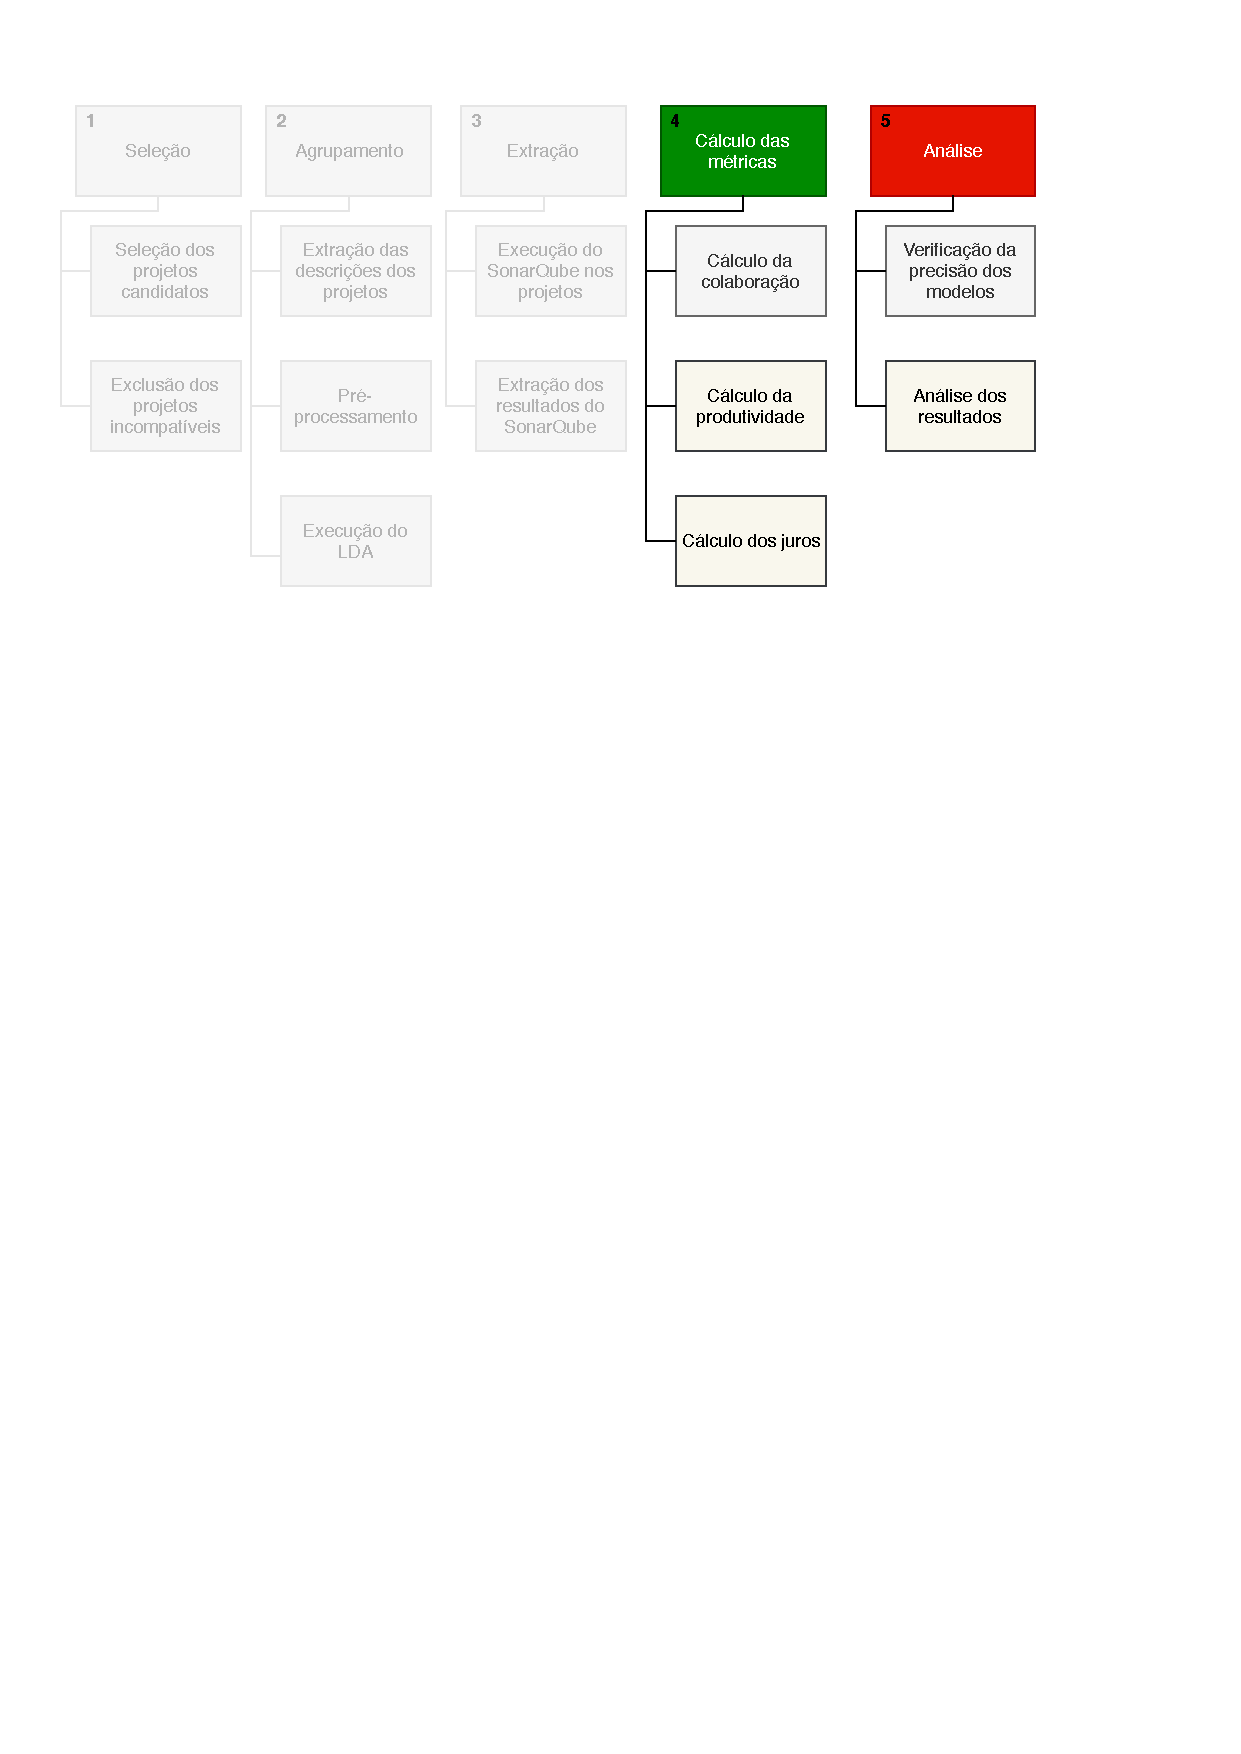
\includegraphics[trim={0.4cm 19.5cm 0cm 1cm},clip]{capitulo_estudo_caso/EtapasMetricas.pdf} 
  \caption{Resumo das etapas do estudo de caso. }
  \label{fig:cap_metodo_resumo_etapas_metricas} 
\end{figure}


\subsection{Cálculo da colaboração}

Conforme descrito anteriormente, consideraremos a colaboração realizada em um projeto como a entrada em nossa estratégia de avaliação de produtividade. Se um projeto tem muita contribuição e pouca evolução, esse projeto será considerado improdutivo. Da mesma forma, se um projeto tem pouca contribuição, mas tem muita evolução, esse projeto será considerado produtivo. 


Conforme descrito no item \ref{cap_metodo:modelos_de_entrada}, utilizaremos três modelos diferentes para calcular a colaboração dos projetos: colaboradores/dia, quantidade de colaboradores e assiduidade e qualidade da colaboração.  A seguir descreveremos detalhes de como os dados de cada um desses modelos foram obtidos.

\subsubsection{Colaboradores/Dia}

Como não tínhamos a disposição à quantidade de horas de contribuição de cada colaborador, tivemos que realizar uma aproximação. Essa aproximação foi realizada substituindo a quantidade de horas pela quantidade de dias em que um colaborador atuou no projeto. A quantidade de dias foi calculada observando a diferença em dias entre a data do primeiro \textit{commit} e a data do último \textit{commit}.

\subsubsection{Quantidade de colaboradores}

Nesse modelo de cálculo da colaboração utilizamos apenas a quantidade de colaboradores em cada projeto. Não foi considerado de nenhuma forma o volume de contribuição de cada colaborador. 

\subsubsection{Assiduidade e qualidade da colaboração}

 Conforme o Capítulo \ref{estimacao:juros}, a colaboração de um projeto será avaliada por meio de um índice que será calculado conforme a equação \ref{eq:cap_calculo_indice_colaboracao}. O valor $A(u)$ representa a assiduidade com o qual o colaborador $u$ contribuiu para o projeto $r$. Já o valor $Q(u)$ representa a qualidade do colaborador $u$. o Conjunto $u(R)$ contém todos os colaboradores que contribuíram no projeto $r$. A seguir descreveremos como foi calculado o $Ic$ de cada projeto.

\begin{equation}
\label{eq:cap_calculo_indice_colaboracao}
I_c(r) =  \sum_{u  \in u(R) } A(u) * Q(u)
\end{equation}

\paragraph{Qualidade de colaboração}


Utilizamos a estratégia descrita no item \ref{cap_modelo_colaboracao_concreto} para calcular a qualidade de cada colaborador. Basicamente, para avaliar a qualidade realizamos uma análise no grafo com os relacionamentos entre colaboradores. Um colaborador será considerado de alta qualidade se ele possui muitos seguidores, contribuiu com projetos relevantes e colaborou com outros colaboradores de qualidade.  O cálculo de colaboração foi implementado na ferramenta GitResearch.  A Figura \ref{fig:codigo_calcula_pagerank} mostra uma das principais funções implementadas.  Nela é realizado o cálculo do \textit{pagerank} tanto dos colaboradores quanto dos projetos. As outras partes da estratégia foram implementadas com o auxílio dos dados disponibilizados pelo GHTorrent. A complexidade dessa implementação está na imensa quantidade de relacionamentos que precisam ser avaliados. Por exemplo, a relação ``seguir'' e ``ser seguido'' de todos os colaboradores que contribuíram com os projetos analisados gerou um grafo de aproximadamente 2 milhões de nós. Com isso, foi necessária a utilização de um hardware potente para que esses relacionamentos fossem calculados em um tempo viável para a realização do estudo de caso. 

 \begin{figure}[H]
  \centering
  \frame{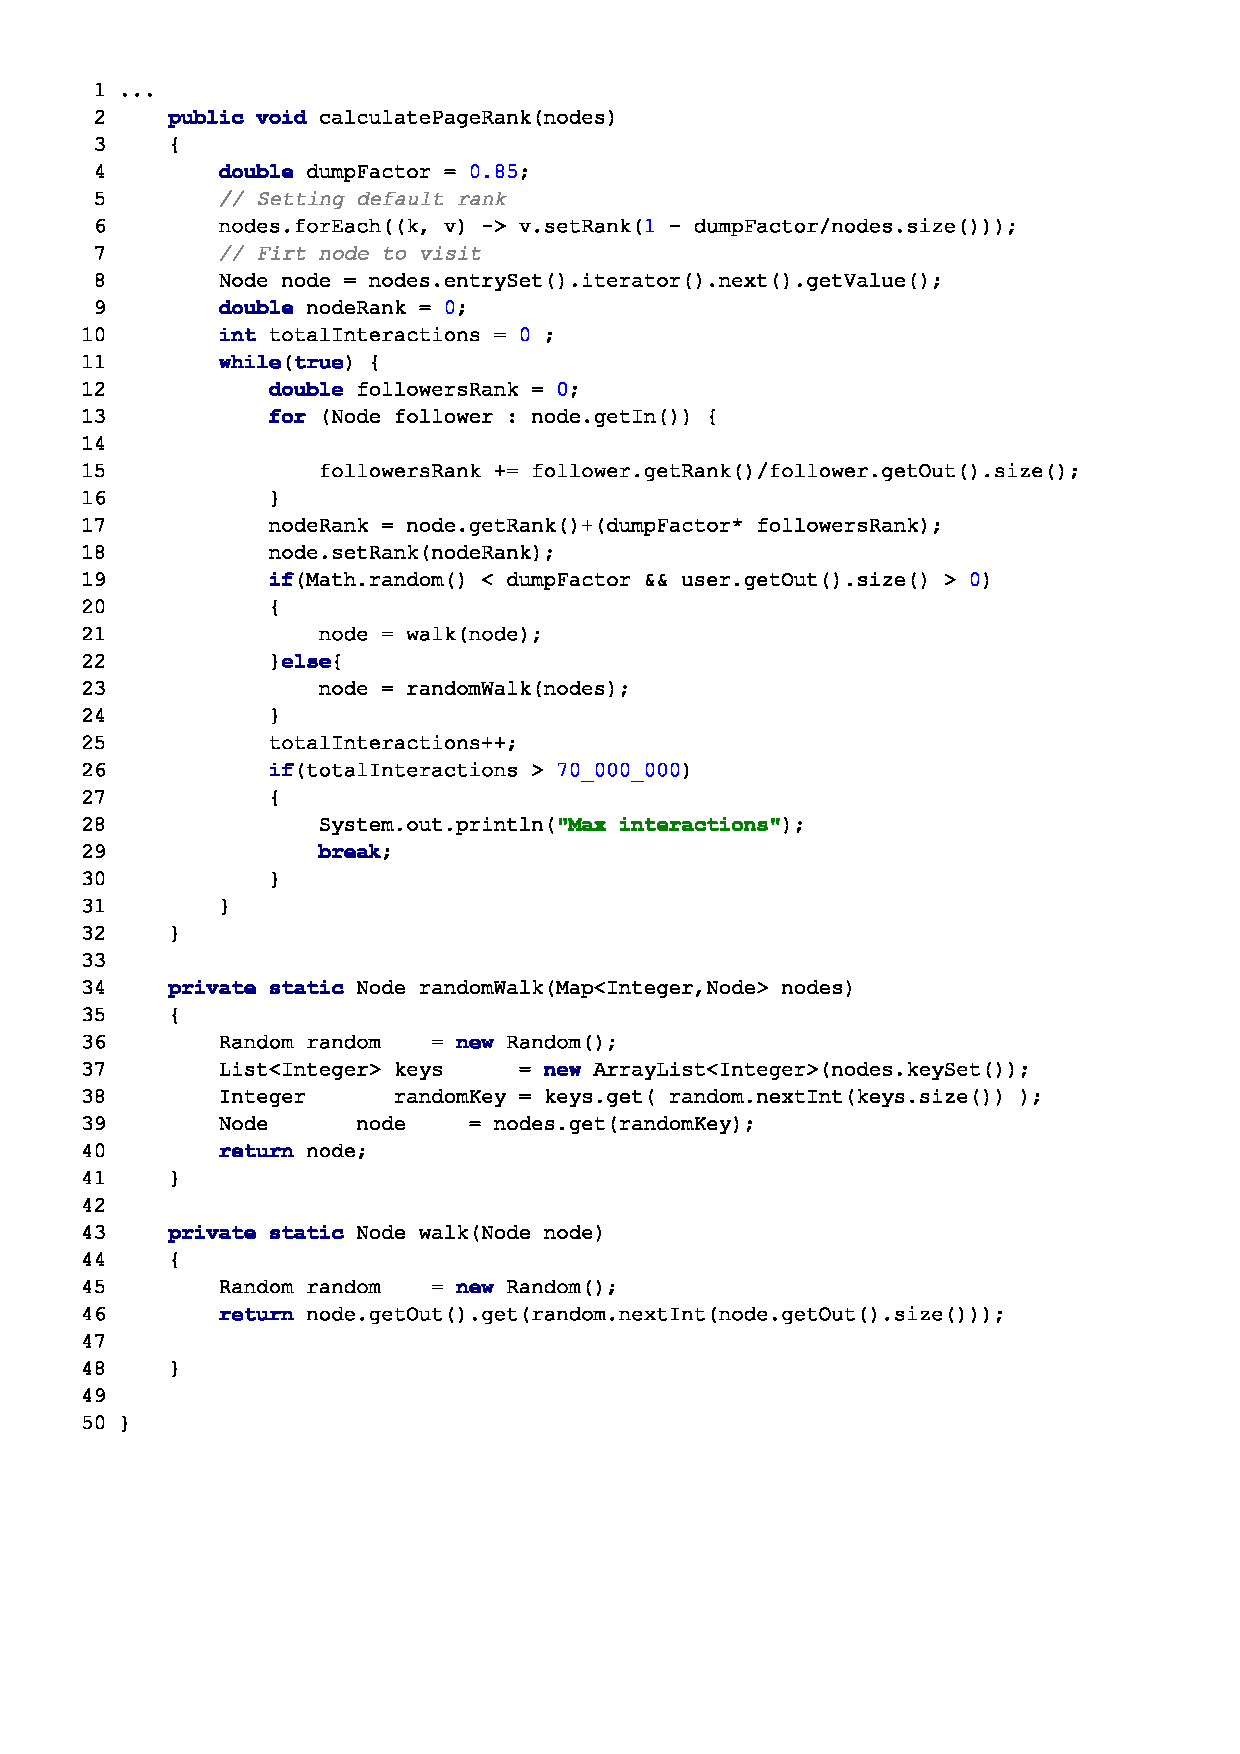
\includegraphics[trim={1cm 4.4cm 2.5cm 1cm},clip]{capitulo_estudo_caso/codigo_page_rank.pdf}} 
  \caption{Código responsável por calcular o pagerank.}
  \label{fig:codigo_calcula_pagerank} 
\end{figure}


\paragraph{Assiduidade}

Analisando o banco de dados de commits disponibilizado pelo projeto GHTorrent até o mês de dezembro de 2017 pudemos calcular que a média de commits que um colaborador faz por dia em um mesmo projeto. O resultado desse cálculo foi: 1,16. Com isso, a assiduidade de um colaborador será calculada utilizando a equação \ref{eq:cap_calculo_assiduidade}. Nessa equação $D_r$ representa a quantidade de dias que um projeto possui desde o primeiro \textit{commit} até o último.  Já a variável $N(u_r)$ representa a quantidade de \textit{commits} que o colaborador $u$ realizou no projeto $r$. Se um colaborador tem uma média diária de \textit{commits} maior do que 1,16 , sua assiduidade no projeto será maior do que 1. Caso contrário, sua assiduidade será menor do que 1. Quanto mais \textit{commits} um colaborador fez em um projeto, maior será a sua assiduidade. 

\begin{equation}
\label{eq:cap_calculo_assiduidade}
A(u_r) =  \frac{N(u_r)}{1,16 * D_r}
\end{equation}

\subsection{Cálculo da produtividade}

A produtividade de cada projeto foi estimada, conforme a sessão \ref{modelo_de_estimacao_produtividade}, observando a relação entre a colaboração estimada e a colaboração real. Como utilizamos três modelos diferentes para avaliar a colaboração, cada projeto também terá três valores para a sua produtividade estimada.

O cálculo da produtividade de cada projeto foi realizado seguindo os seguintes etapas para cada modelo de colaboração:

\begin{enumerate}
\item Foi calculada a colaboração real do projeto de acordo com o modelo de colaboração.
\item Foi realizada uma regressão linear múltipla tendo como variável dependente a colaboração real do projeto e como variáveis independentes a quantidade de linhas de código, quantidades de \textit{watchers} e a quantidade de \textit{pull requests}.
\item Utilizando os coeficientes obtidos pela regressão linear, foi calculado o valor ajustado para a medida de colaboração de cada projeto. Esse valor ajustado corresponde ao valor esperado de contribuição para que tivessem sido alcançados os resultados do projeto. Um projeto produtivo é aquele com um valor ajustado de colaboração maior do que o valor real de colaboração.
\item Foi calculada a produtividade estimada de cada projeto utilizando a equação \ref{eq:model_capitulo_estudo}.
\end{enumerate}

\begin{equation}
\label{eq:model_capitulo_estudo}
  Productivity = AdjustedSize/Effort
\end{equation}


\section{Cálculo dos juros}


Os juros foram calculados por tópico seguindo uma adaptação do procedimento descrito na sessão \ref{estimacao_juros_por_aproximacao}:

\begin{enumerate}
\item Os projetos de cada tópico foram separados em duas partições, representando os cenários descritos no Capítulo \ref{estimacao:juros}: 
   \begin{itemize}
      \item \textbf{Sem dívida técnica}: Projetos que estivessem entre os 5\% com menos dívida técnica. A quantidade de dívida técnica de cada projeto foi calculada como a média das cincos médições do campo SQALE\_DEBT\_INDEX. Conforme apresentado na Tabela \ref{table:metricas_sonar}, esse campo armazena a proporção entre dívida técnica e tamanho de um projeto. 
      \item \textbf{Com dívida técnica}: Todos os outros projetos.
   \end{itemize}
  \item Foi calculada a produtividade média dos projetos em cada partição.
  \item Os juros foram calculados como a diferença entre a produtividade média das duas partições.
\end{enumerate}




\section{Análise}

 \begin{figure}[H]
  \centering
  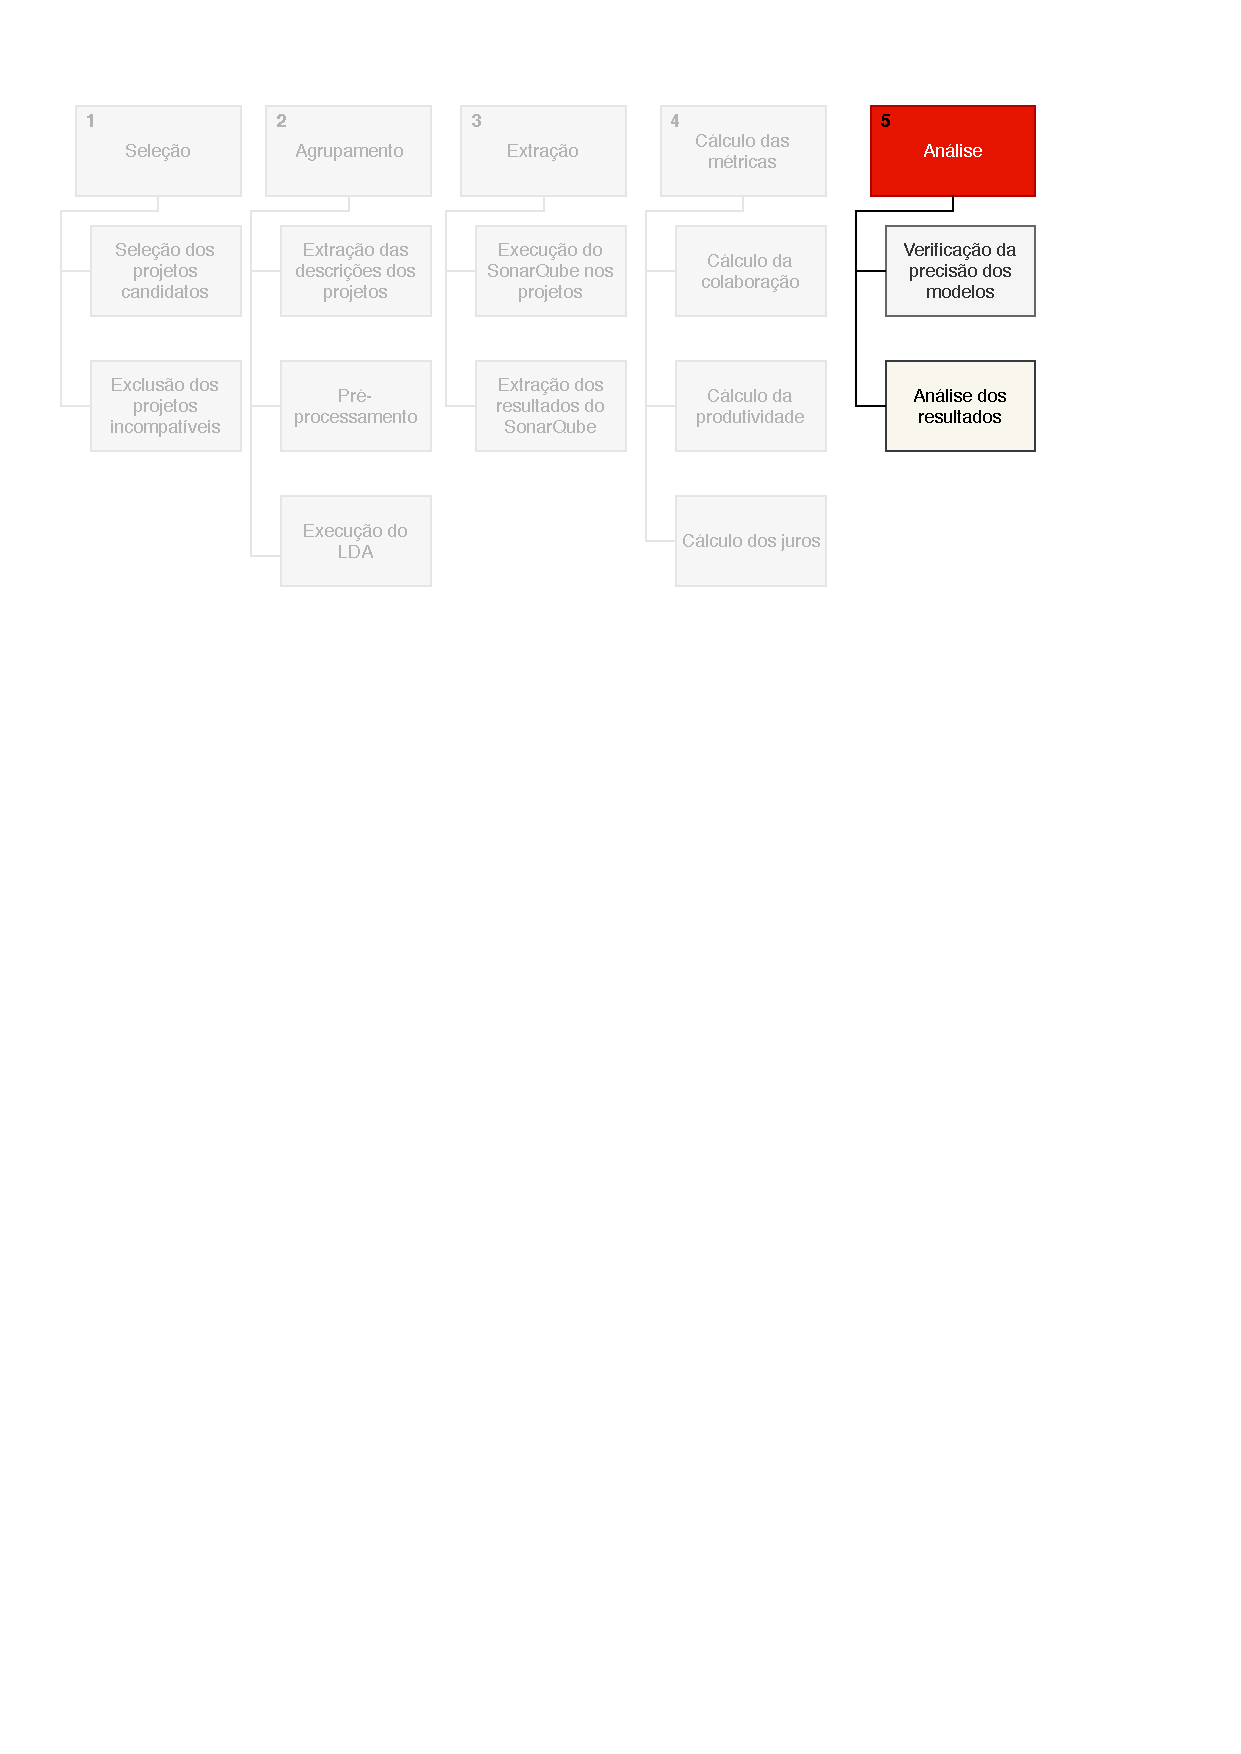
\includegraphics[trim={0.4cm 19.5cm 0cm 1cm},clip]{capitulo_estudo_caso/EtapasAnalise.pdf} 
  \caption{Resumo das etapas do estudo de caso. }
  \label{fig:cap_metodo_resumo_etapas_extracao} 
\end{figure}

Para avaliarmos os dados obtidos durante o estudo de caso realizaremos uma análise exploratória. Serão apresentadas diversas estatísticas e visualizações com o intuito de fornecer um panorama a respeito das informações encontradas. Todas as métricas foram obtidas em cinco pontos diferentes da evolução dos projetos. Entretanto,  quando não explicitado o contrário, todas as tabelas e gráficos são relativos aos valores mais recentes, isto é, foram criadas utilizando os dados da última leitura realizada. 



\subsection{Análise dos resultados}

A tabela \ref{tabela_sumario_metricas} apresenta um resumo com as principais medidas descritivas das métricas extraídas dos projetos. Existem alguns aspectos interessantes na Tabela \ref{tabela_sumario_metricas}. Um deles é a existência de métricas nas quais o valor mínimo encontrado foi zero. Ao analisarmos esses projetos com valor zero nessas métricas, pudemos observar que isso ocorreu devido ao fato de esses projetos terem sido descontinuados recentemente. Com isso, o código fonte na última leitura que realizamos foi apagado ou drasticamente diminuído.  

Outra aspecto relevante da Tabela \ref{tabela_sumario_metricas} é o comportamento da métrica \textbf{sqale debt ratio}. Conforme a Tabela \ref{table:metricas_sonar}, essa métrica armazena a proporção entre o tamanho do software e a sua dívida técnica. Como podemos ver, essa métrica tem um desvio padrão próximo a 1. Isso indica que não há uma grande variação da proporção da dívida técnica entre os projetos.  Entretanto, o valor máximo é de 12,4. Isso é um indício da existência de \textit{outliers}. De acordo com Hawkins et al. \cite{hawkins1980identification}, um \textit{outlier} é um valor que se afasta demasiadamente dos demais de uma série ou é um valor medido incorretamente. Para verificarmos se não houve alguma falha na medição, realizamos uma análise dos 30 projetos com os maiores valores nessa métrica. Em todos os casos, o valor medido anteriormente foi confirmado. Analisando o código-fonte desses projetos, chegamos às seguintes razões para o elevado nível de dívida técnica:

\begin{itemize}
\item A existência de códigos de teste com um nível de qualidade muito inferior ao restante do software.
\item A existência de arquivos e códigos descontinuados(\textit{deprecated}).
\item  Uma acentuada despreocupação dos colaboradores em seguir as boas práticas do desenvolvimento de software.
\end{itemize}


\begin{table}[H]
\scriptsize                 
\def\arraystretch{1.3}%
\centering
\begin{tabular}{|l|l|l|l|l|l|l|l|}
\hline
 &\textbf{Des. Padrão} & \textbf{Mín.}      & \textbf{1\textsuperscript{o} Quart.}  & \textbf{Mediana} & \textbf{Média}    & \textbf{3\textsuperscript{o}. Quart.}    & \textbf{Máx.}              \\ \hline
\textit{\textbf{CODE\_SMELLS }} & 10736,52     &0,0  &  637,2  & 1781,5 &  4897,7 &  4613,2 & 176454     \\ \hline
\textit{\textbf{COGNITIVE\_COMPLEXITY }} & 24376,92 & 0   & 1378    & 4176 & 12004 & 12174 & 440187  \\ \hline
\textit{\textbf{COMMENT\_LINES }} & 41883,15   & 5    & 1624      & 5083   &  17419   &  15624   & 690566     \\ \hline
\textit{\textbf{COMMENT\_LINES\_DENSITY}} & 8,274049    & 0,10  &  7,60    & 12,10     & 13,58    & 18,20    & 64,10  \\ \hline
\textit{\textbf{COMPLEXITY  }}   & 27665,5  & 0 & 2507  & 6244   & 15453  & 16386  & 413387 \\ \hline
\textit{\textbf{DIRECTORIES}} & 275,1348    & 1    & 34   & 79     & 169,2   & 183,8     & 3743,0    \\ \hline
\textit{\textbf{DUPLICATED\_LINES}}   & 44410,89    & 0 & 779  & 3155    & 15926     & 11737    & 577213      \\ \hline
\textit{\textbf{DUPLICATE\_LINES\_DENSITY}}   & 8,683636   & 0  & 2,400    & 5    & 7,367    & 8,90   & 97  \\ \hline
\textit{\textbf{DUPLICATED\_BLOCKS}}   & 3415,468   & 0  & 41   & 169    &   974,7  & 647,8    & 79718   \\ \hline
\textit{\textbf{DUPLICATED\_FILES  }}   & 363,5063    & 0  & 17    & 57     & 166,5    & 159    &  6078 \\ \hline
\textit{\textbf{FILES }}   & 1523,965    & 1  & 208    & 458,5     & 963,1   & 1056,2   & 20849  \\ \hline
\textit{\textbf{FUNCTIONS}}   & 14230,68    & 2  & 1468    & 3453     & 8226    & 8561    & 168295  \\ \hline
\textit{\textbf{NLOC}}   & 155979,5    & 30  & 15973   & 37429     & 91572    & 98373    & 1996351  \\ \hline
\textit{\textbf{SQALE\_DEBT\_RATIO}}   & 0,9809708    & 0,10  &  1,10    & 1,50    & 1,73    & 2,10    & 12,40   \\ \hline
\textit{\textbf{SQALE\_RATING}}   & 0,1121445    & 1  & 1    & 1     & 1,01   & 1    & 3  \\ \hline
\textit{\textbf{STATEMENTS }}   & 71565,78    &0  & 6401    & 15784     & 40319    & 43096    & 912227  \\ \hline
\textit{\textbf{VIOLATIONS }}   & 11374,37    & 0  & 708    & 1935   & 5319    & 5057    & 176844  \\ \hline

\end{tabular}
\caption{Sumário das medidas descritivas das métricas obtidas dos projetos.}
\end{table}
\label{tabela_sumario_metricas}


\subsection{Distruição dos projetos por tópicos}


Os projetos foram distribuídos em 30 tópicos após a aplicação do LDA. A Figura \ref{fig:projetos_por_topicos} apresenta a quantidade de projetos em cada um dos tópicos. Podemos observar que não houve uma distruição uniforme dos projetos em cada tópico. Alguns tópicos como o 13 tiveram uma quantidade maior de projetos. Enquanto isso, alguns tópicos como o 28 e 10 tiveram uma quantidade significativamente menor de projetos. Existem algumas razões para essa variação:

\begin{itemize}
\item A existência de alguns assuntos que genuinamente possuem mais projetos relacionados no GitHub. Esse é o caso, por exemplo, do tópico 9 que é o segundo maior tópico obtido. Na Tabela \ref{table:topicos_lda} podemos ver as palavras presentes nesse tópico e com isso, inferir que os projetos presentes nele são relacionados a aplicações para a internet. Isso explica a quantidade maior de projetos já que esse é um domínio popular. 
\item As deficiências na utilização do LDA para a categorização de projetos de software. No caso do tópico 13, uma das possíveis razões para o seu alto número de projetos é a quantidade de palavras muito comuns que ele possui. De acordo com a Tabela \ref{table:topicos_lda}, as duas primeiras palavras desse tópico são \textit{issue} e \textit{contribution}. Essas palavras são demasiadamente comuns na descrição de projetos de software livre. Isso fez com que o tópico 13 fosse o tópico com o maior número de projetos.
\end{itemize} 


Para facilitar a visualização do comportamento dos dados  realizamos um agrupamento dos tópicos por domínio conforme mostrado na Tabela \ref{table_cap_estudo_topicos_dominios}. Esse agrupamento foi feito observando as palavras de cada um dos tópicos e analisando alguns dos projetos de cada tópico. Foram identificados 7 domínios: Aplicação, Gerenciamento de Dados, Ferramenta, Arcabouço, Middleware, Biblioteca e Outro. Todos os projetos que não puderam ser classificados foram colocados no domínio Outro. A Figura \ref{fig:projetos_por_dominio} apresenta a distrubuição dos projetos dentro dos 7 domínios. É possível notar que houve uma distribuição mais uniforme dos projetos quando é realizado o agrupamento dos tópicos em domínios. 



 \begin{figure}[H]
  \centering
  \frame{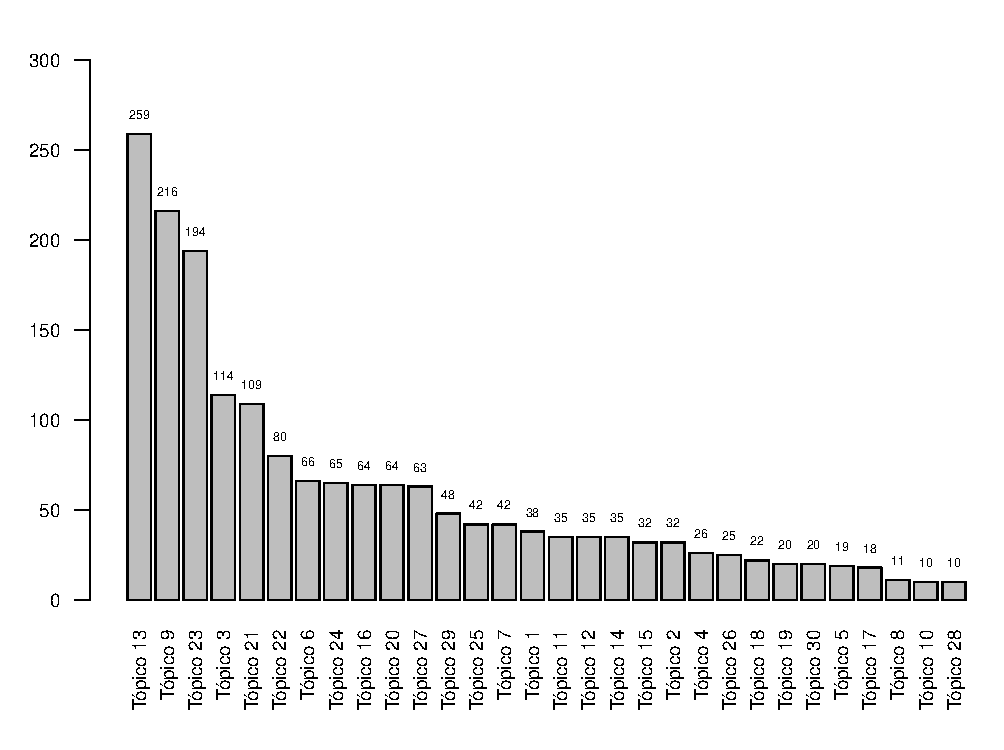
\includegraphics[trim={0cm 0cm 0cm 0cm},clip]{capitulo_estudo_caso/analise_exploratoria/projetos_por_topicos.pdf}} 
  \caption{Quantidade de projetos por tópico do LDA.}
  \label{fig:projetos_por_topicos} 
\end{figure}

\begin{table}[H]
\small 
\def\arraystretch{3}% 
\begin{tabular}{|l|l|l|l|}
\hline
\textbf{Domínio}       & \pbox{1cm}{\textbf{Tópicos}}  &  \pbox{5cm}{\textbf{Descrição}}                                     &  \pbox{4cm}{\textbf{Exemplos}}                               \\ \hline
Aplicação              & \pbox{1cm}{1, 4, 9, 10, 17, 22, 28} &  \pbox{5cm}{Programas voltados para o usuário final.}                &  \pbox{4cm}{Morphium, XPrivacy, Mule, SilenceIM}              \\ \hline
Gerenciamento de dados & \pbox{2cm}{2, 5, 12, 21, 24, 25}   &  \pbox{5cm}{Aplicações para processamento e gerenciamento de dados.} &  \pbox{4cm}{Asterixdb, Cassandra, Hive, Hibernate-ogm}          \\ \hline
Ferramenta             & \pbox{1cm}{3, 23, 30}           &  \pbox{5cm}{Ferramentas de desenvolvimento.}                         &  \pbox{4cm}{Cloudify, Kotlin-eclipse, Bitcoinj, Pentaho-kettle} \\ \hline
Arcabouço              & \pbox{1cm}{6, 18, 19, 20, 27}     &  \pbox{5cm}{Arcabouços para o desenvolvimento de software.}          &  \pbox{4cm}{Spring-cloud-commons, Guava, arquillian-cube}    \\ \hline
Middleware             & \pbox{1cm}{7, 14}              &  \pbox{5cm}{Aplicações voltadas para a infraestrutura.}              &  \pbox{4cm}{Docker-maven-plugin, s3proxy, aws-mock}          \\ \hline
Biblioteca             & \pbox{1cm}{8, 15, 16, 26}        & \pbox{5cm}{Bibliotecas de códigos.}                                 &  \pbox{4cm}{Tnt4j, Swagger-codegen, java-client-api}         \\ \hline
Outro                  & \pbox{1cm}{11, 13, 29}          & \pbox{5cm}{Não puderam ser classificados.}                          &  \pbox{4cm}{Abstools, react-native, RxJava, vraptor4}        \\ \hline
\end{tabular}
\caption{Tópicos agrupados em domínios.}
\end{table}
\label{table_cap_estudo_topicos_dominios}




 \begin{figure}[H]
  \centering
  \frame{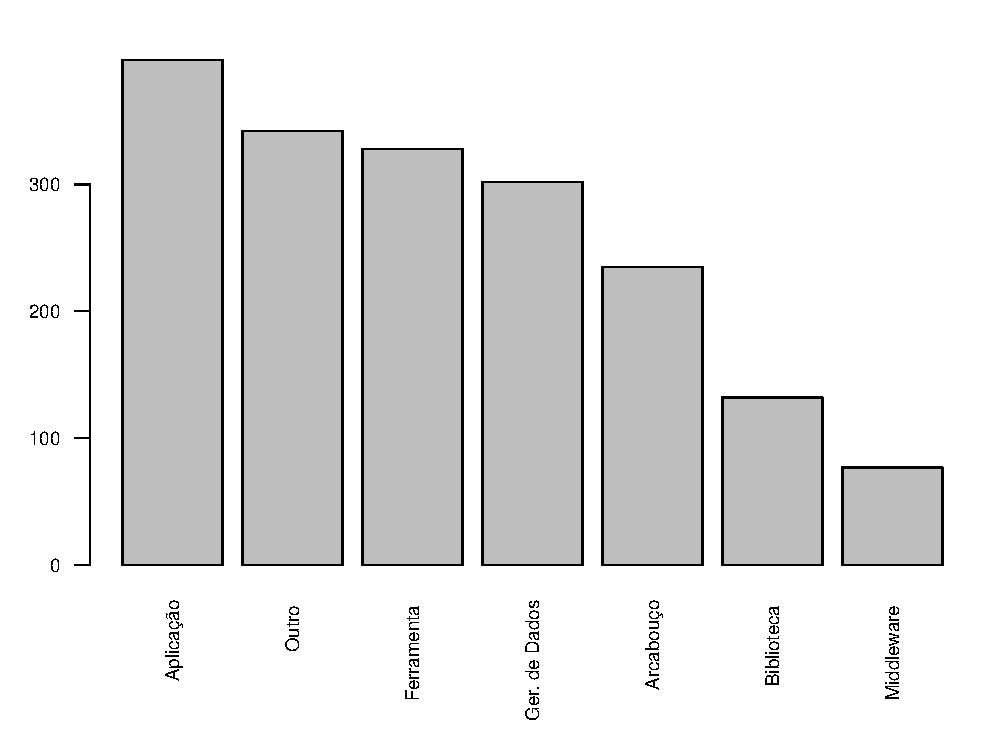
\includegraphics[trim={0cm 0cm 0cm 0cm},clip]{capitulo_estudo_caso/analise_exploratoria/projetos_por_dominio.pdf}} 
  \caption{Quantidade de projetos por domínio.}
  \label{fig:projetos_por_dominio} 
\end{figure}


\subsection{Dívida técnica}

A Figura \ref{fig:boxplot_divida_tecnica} apresenta um \textit{boxplot} a respeito da distribuição da dívida técnica em todos os projetos do estudo de caso. Conforme pode ser visto, a mediana se aproxima de 1,5. Isso vai de encontro a resultados de pesquisas anteriores em que o valor da mediana era próximo de três\cite{de2017technical}. As Figura \ref{fig:divida_por_topico} e \ref{fig:divida_por_dominio} apresentam \textit{boxplots} com a distribuição do valor da dívida técnica dos projetos agrupados por tópicos e domínios, respectivamente. 


 \begin{figure}[H]
  \centering
  \frame{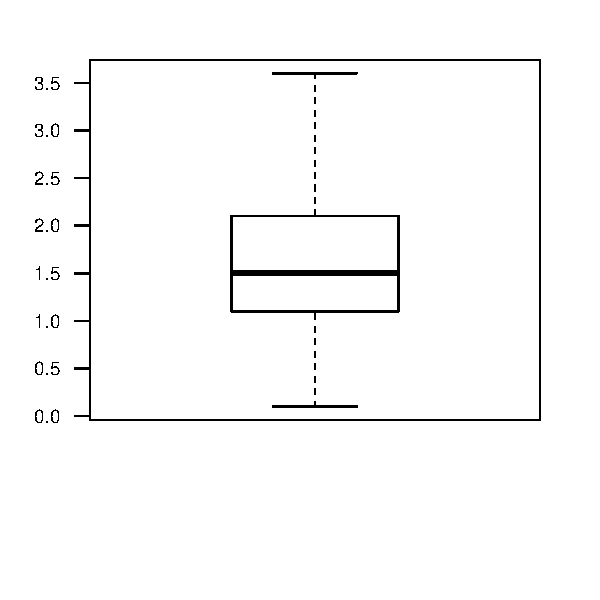
\includegraphics[trim={0cm 2cm 0cm 0cm},clip]{capitulo_estudo_caso/analise_exploratoria/divida_tecnica_sozinha.pdf}} 
  \caption{Dívida técnica.}
  \label{fig:boxplot_divida_tecnica} 
\end{figure}

 \begin{figure}[H]
  \centering
  \frame{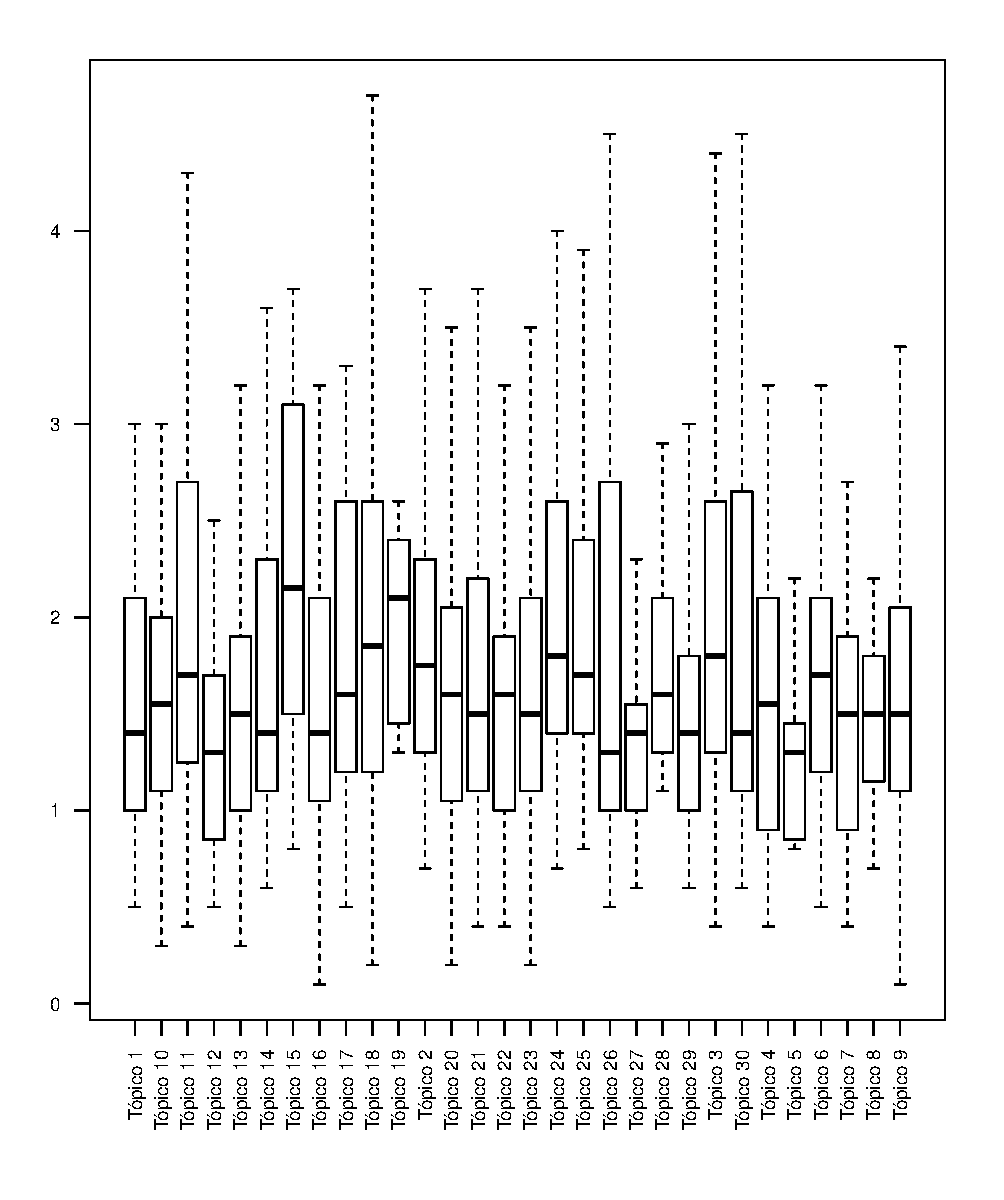
\includegraphics[trim={0cm 0cm 0cm 0cm},clip]{capitulo_estudo_caso/analise_exploratoria/divida_tecnica_por_topico.pdf}} 
  \caption{Dívida técnica por tópico.}
  \label{fig:divida_por_topico} 
\end{figure}

 \begin{figure}[H]
  \centering
  \frame{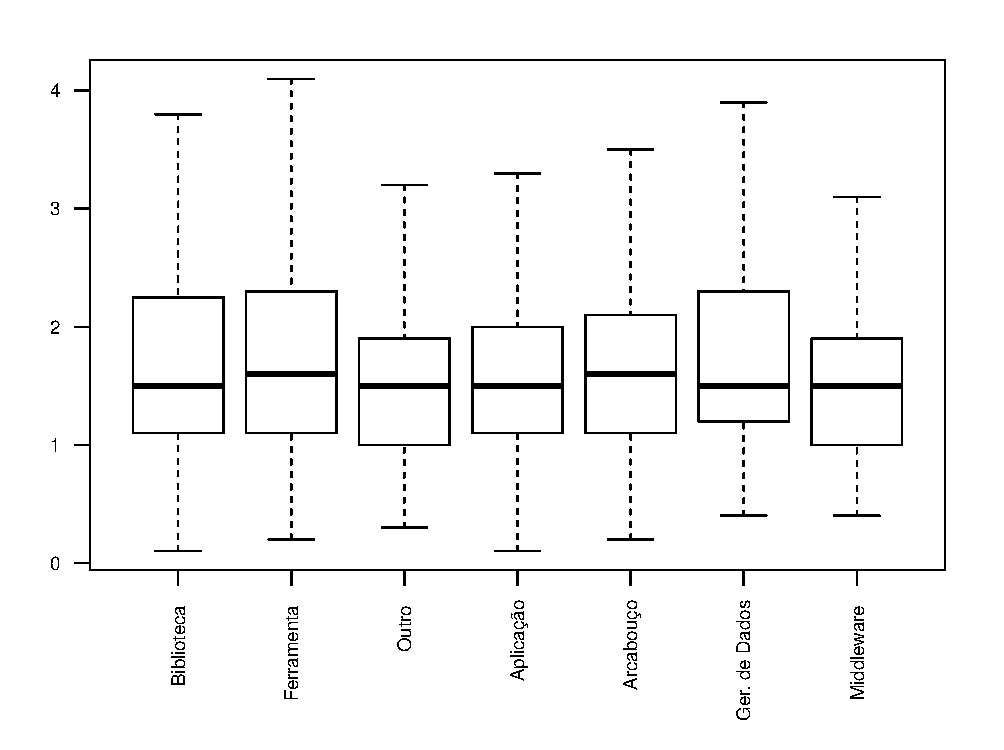
\includegraphics[trim={0cm 0cm 0cm 0cm},clip]{capitulo_estudo_caso/analise_exploratoria/divida_tecnica_por_dominio.pdf}} 
  \caption{Dívida técnica por domínio.}
  \label{fig:divida_por_dominio} 
\end{figure}


Na Figura \ref{fig:histograma_leitura_divida} é apresentado um histograma, com a quantidade de projetos por intervalo de dívida técnica, para cada leitura realizada. 

 \begin{figure}[H]
  \centering
  \frame{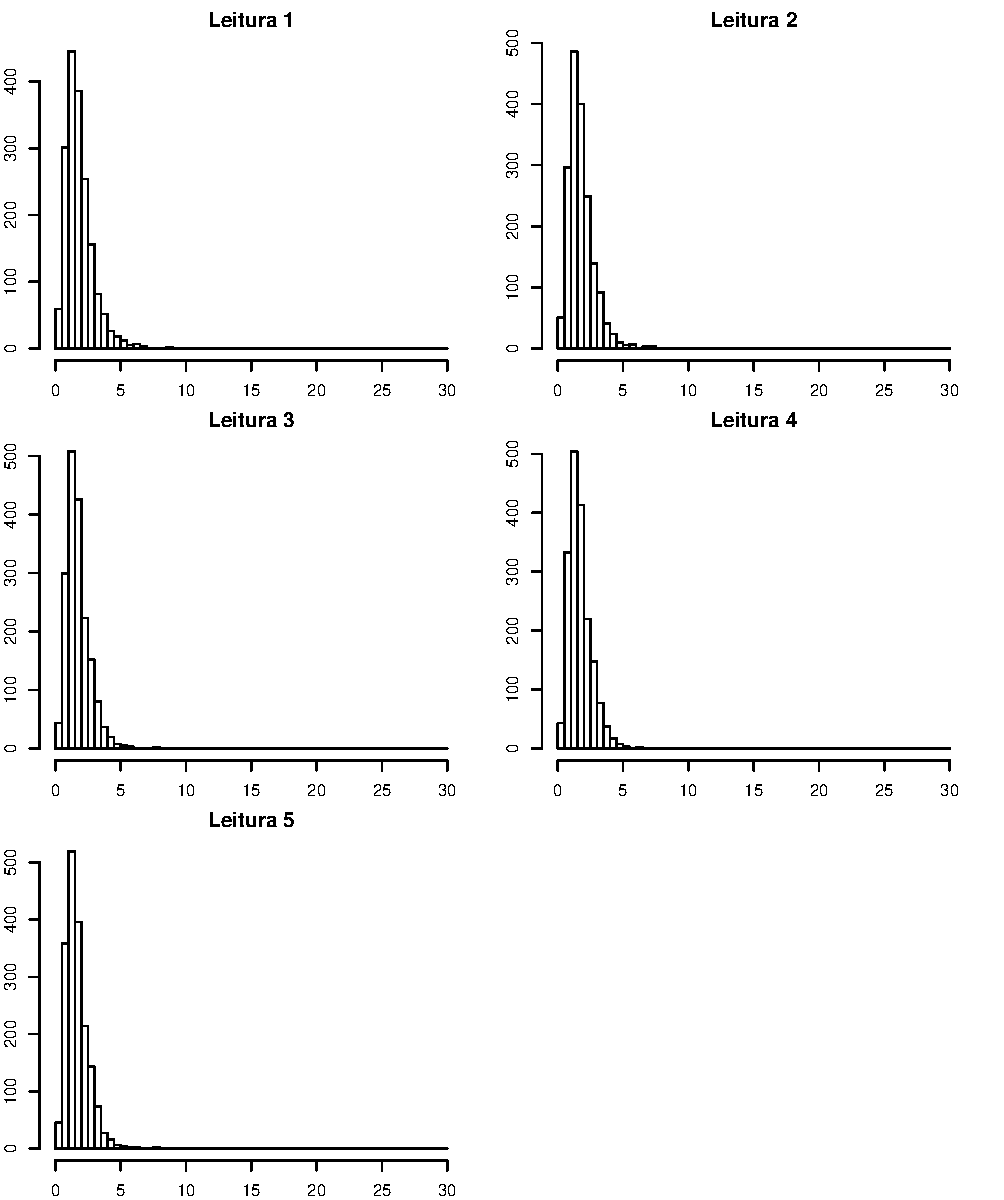
\includegraphics[trim={0cm 0cm 0cm 0cm},clip]{capitulo_estudo_caso/analise_exploratoria/histograma_divida_leitura.pdf}} 
  \caption{Dívida técnica por domínio.}
  \label{fig:histograma_leitura_divida} 
\end{figure}


Por termos feito cinco leituras em períodos diferentes da evolução dos projetos, podemos analisar a evolução da dívida técnica nos mesmos. A Figura \ref{fig:evolucao_por_dominio} apresenta a evolução da dívida técnica nos projetos agrupados por domínio. É possível notar que há predominantemente uma tendência de queda. Ou seja, à medida que os projetos evoluem, o nível da dívida técnica cai. Entretanto, essa variação temporal é pequena.  Um exemplo são os projetos do domínio \textbf{aplicação}. Inicialmente a média da dívida técnica desses projetos foi de aproximadamente 1,9. Entretanto, com o passar do tempo, essa média caiu para 1,65. 



 \begin{figure}[H]
  \centering
  \frame{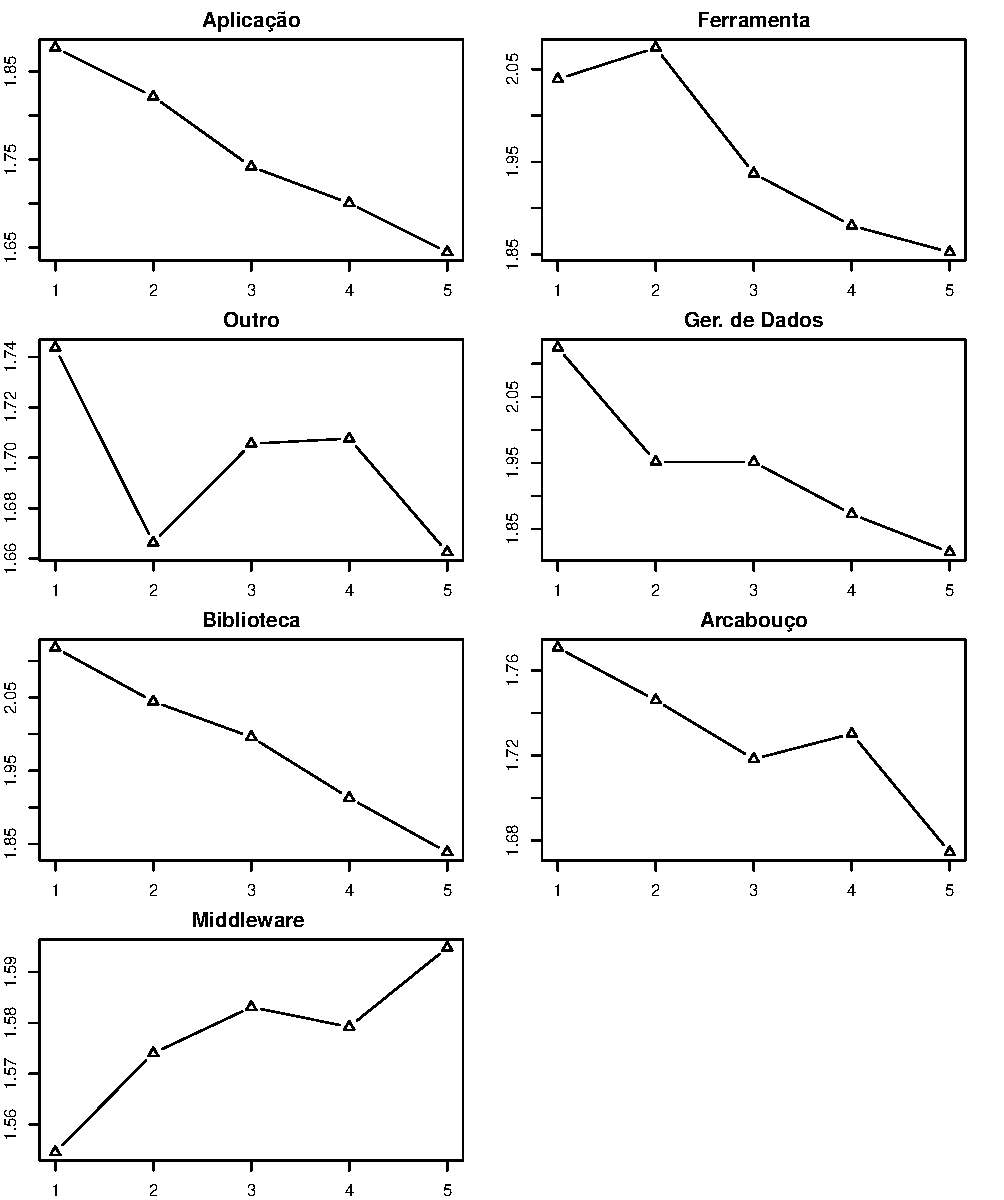
\includegraphics[trim={0cm 0cm 0cm 0cm},clip]{capitulo_estudo_caso/analise_exploratoria/evolucao_divida_dominio.pdf}} 
  \caption{Evolução da dívida técnica por domínio.}
  \label{fig:evolucao_por_dominio} 
\end{figure}



\subsection{Tamanho dos projetos}

A Figura \ref{fig:histograma_nloc} apresenta um histograma com o número de projetos por faixa de tamanho. É possível verificar que grande parte dos projetos tem menos do que quinhentas mil linhas de código-fonte. Porém, existem alguns projetos acentuadamente maiores e que ultrapassam as cem mil linhas. As Figuras \ref{fig:histograma_nloc} e \ref{fig:linhas_codigo_dominio} apresentam \textit{boxplots} com a distribuição da quantidade de linhas de código agrupadas por tópicos e domínios respectivamente. Já a Figura \ref{fig:evolucao_linhas_codigo_dominio} apresenta a evolução da quantidade de linhas de código entre as leituras realizadas. Como esperado, há uma tendência de crescimento já que a medida que o software evoluiu, mais linhas de código são inseridas. 


 \begin{figure}[H]
  \centering
  \frame{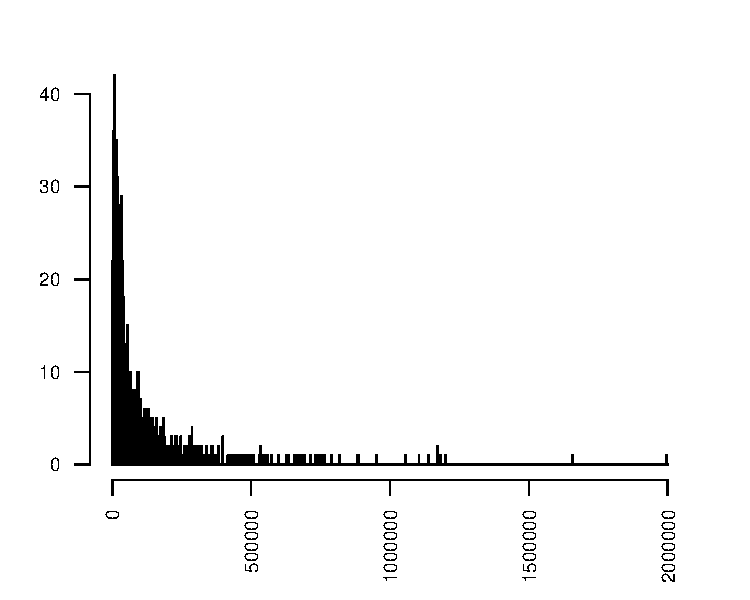
\includegraphics[trim={0cm 0cm 0cm 0cm},clip]{capitulo_estudo_caso/analise_exploratoria/histograma_nloc.pdf}} 
  \caption{Frequência de projetos por intervalo de número de linhas de código.}
  \label{fig:histograma_nloc} 
\end{figure}



 \begin{figure}[H]
  \centering
  \frame{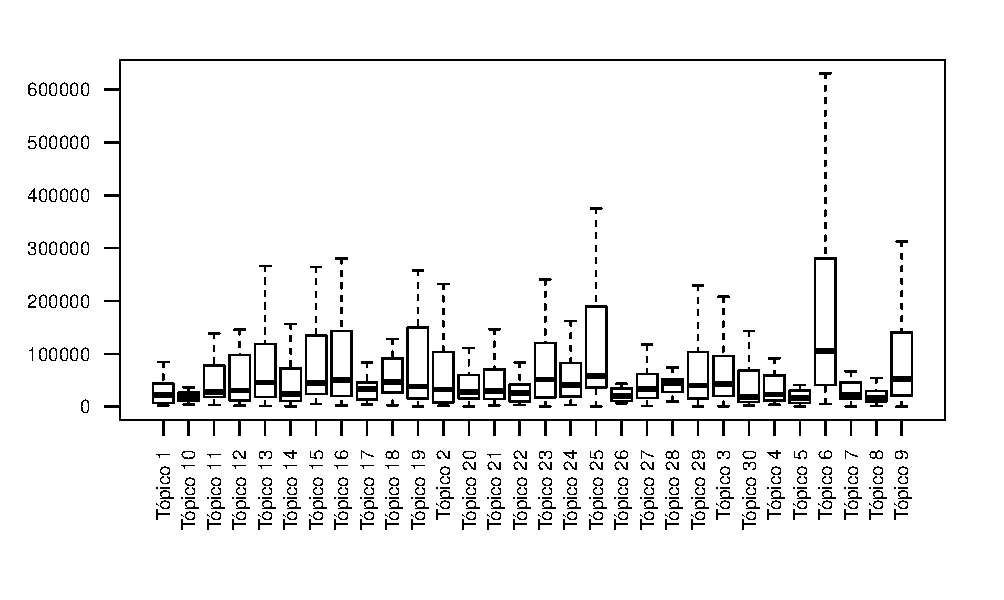
\includegraphics[trim={0cm 0cm 0cm 0cm},clip]{capitulo_estudo_caso/analise_exploratoria/linhas_de_codigo_por_topico.pdf}} 
  \caption{Dívida técnica por domínio.}
  \label{fig:linhas_codigo_topico} 
\end{figure}

 \begin{figure}[H]
  \centering
  \frame{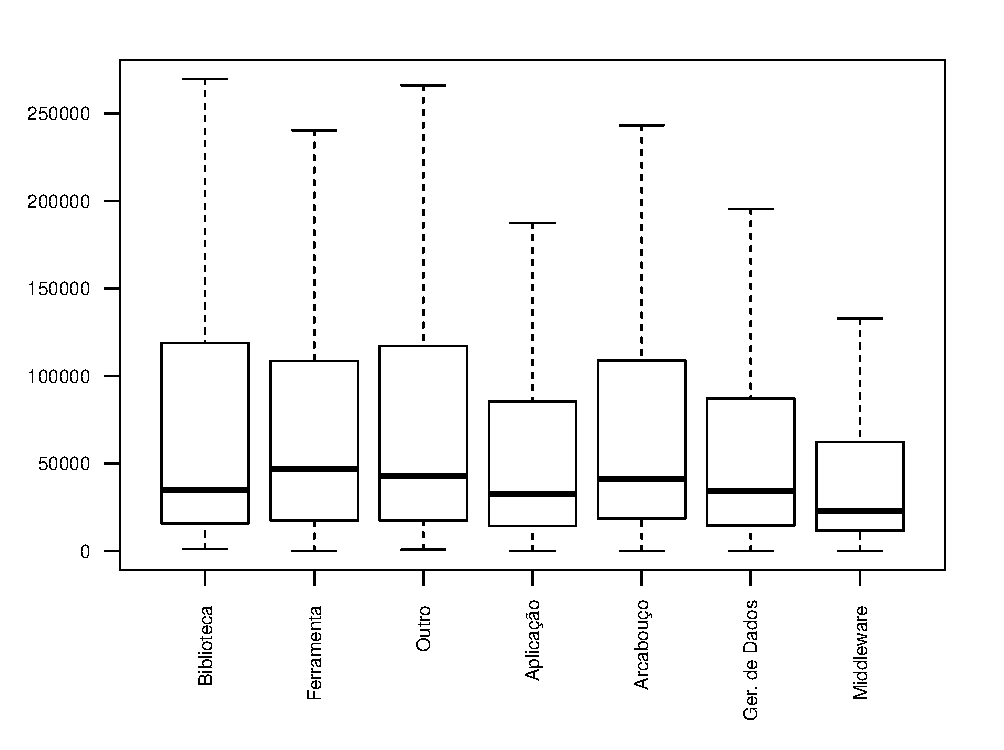
\includegraphics[trim={0cm 0cm 0cm 0cm},clip]{capitulo_estudo_caso/analise_exploratoria/linhas_de_codigo_por_dominio.pdf}} 
  \caption{Dívida técnica por domínio.}
  \label{fig:linhas_codigo_dominio} 
\end{figure}


 \begin{figure}[H]
  \centering
  \frame{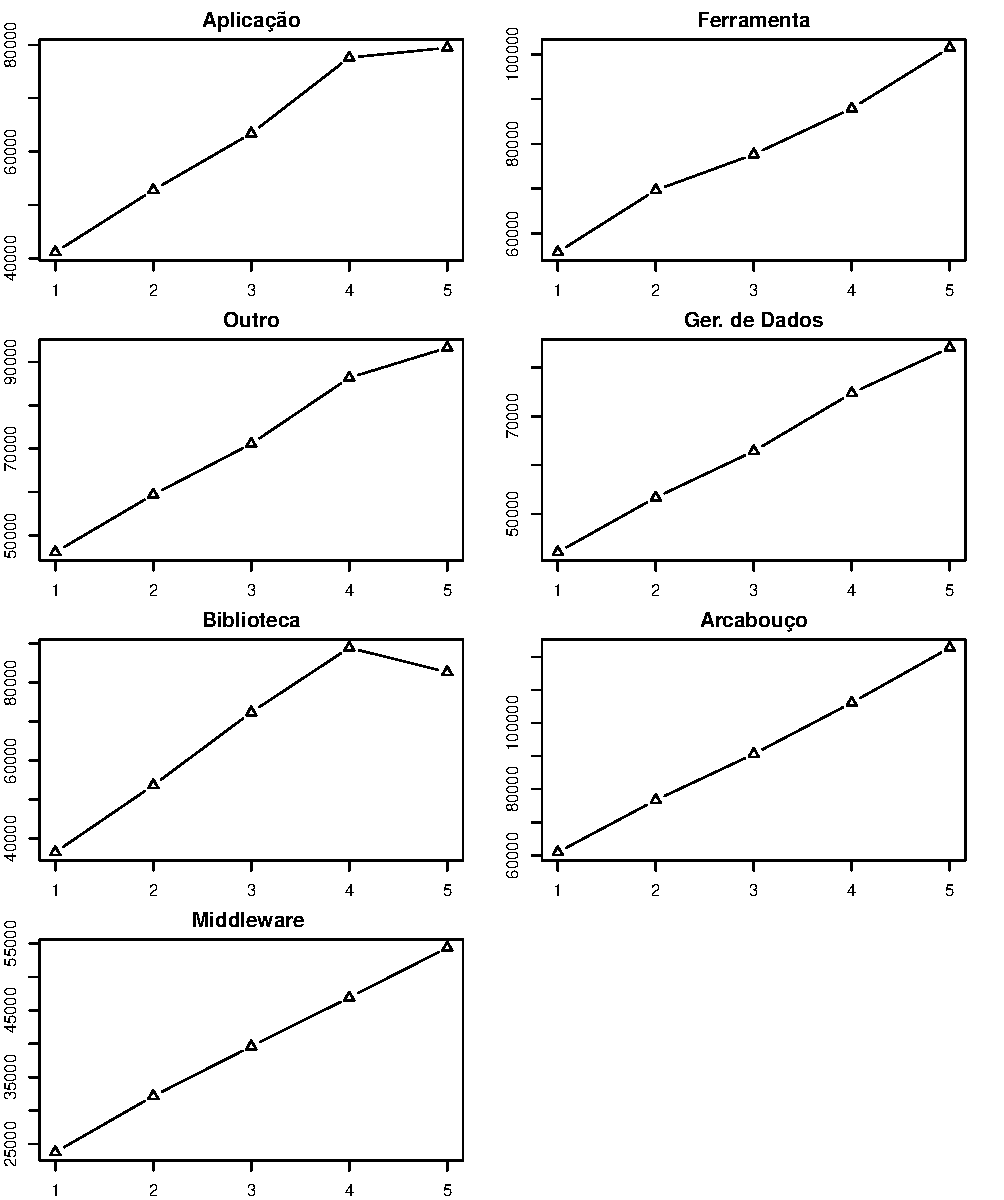
\includegraphics[trim={0cm 0cm 0cm 0cm},clip]{capitulo_estudo_caso/analise_exploratoria/evolucao_linhas_de_codigo_dominio.pdf}} 
  \caption{Dívida técnica por domínio.}
  \label{fig:evolucao_linhas_codigo_dominio} 
\end{figure}


\subsection{Correlações entre a dívida técnica e as métricas de tamanho}

Nas Figuras \ref{fig:correlacao_divida_linhas_codigo},  \ref{fig:correlacao_divida_watchers} e \ref{fig:correlacao_divida_pull_request} foram exibidas as correlações entre a dívida técnica e as variáveis linhas de código, \textit{watchers} e \textit{pull requests}, respectivamente. Conforme pode ser notado, apenas há indício de correlação com a variável linhas de código. Ainda assim, essa correlação, medida de forma geral, sem separação por domínios, é de apenas 0,1164773  com \textit{p-value} de 0,0000006545. 

 \begin{figure}[H]
  \centering
  \frame{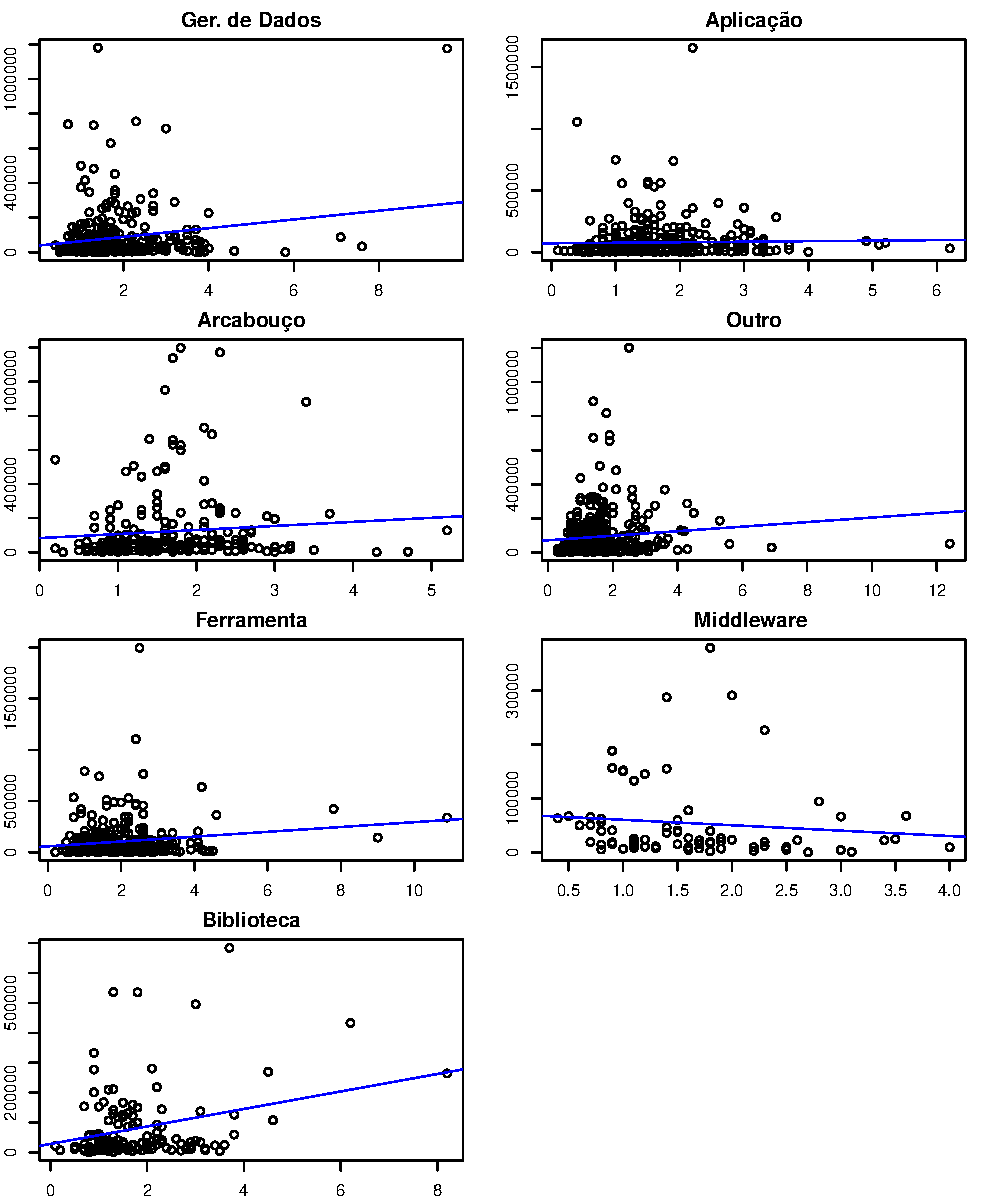
\includegraphics[trim={0cm 0cm 0cm 0cm},clip]{capitulo_estudo_caso/analise_exploratoria/correlacao_divida_nloc.pdf}} 
  \caption{Correlação entre a dívida técnica e a quantidade de linhas de código.}
  \label{fig:correlacao_divida_linhas_codigo} 
\end{figure}

 \begin{figure}[H]
  \centering
  \frame{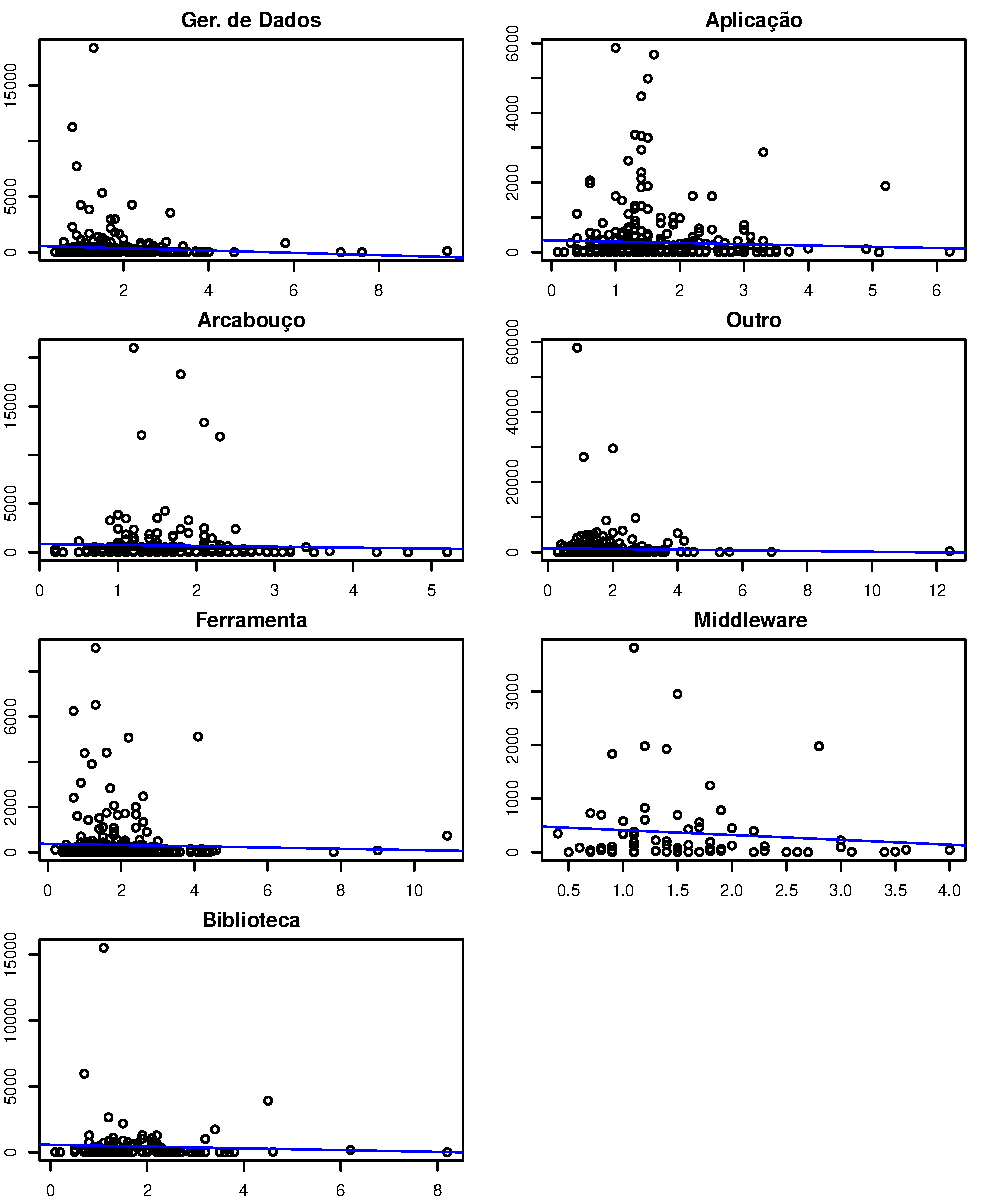
\includegraphics[trim={0cm 0cm 0cm 0cm},clip]{capitulo_estudo_caso/analise_exploratoria/correlacao_divida_watchers.pdf}} 
  \caption{Correlação entre a dívida técnica e a quantidade de \textit{watchers}.}
  \label{fig:correlacao_divida_watchers} 
\end{figure}


 \begin{figure}[H]
  \centering
  \frame{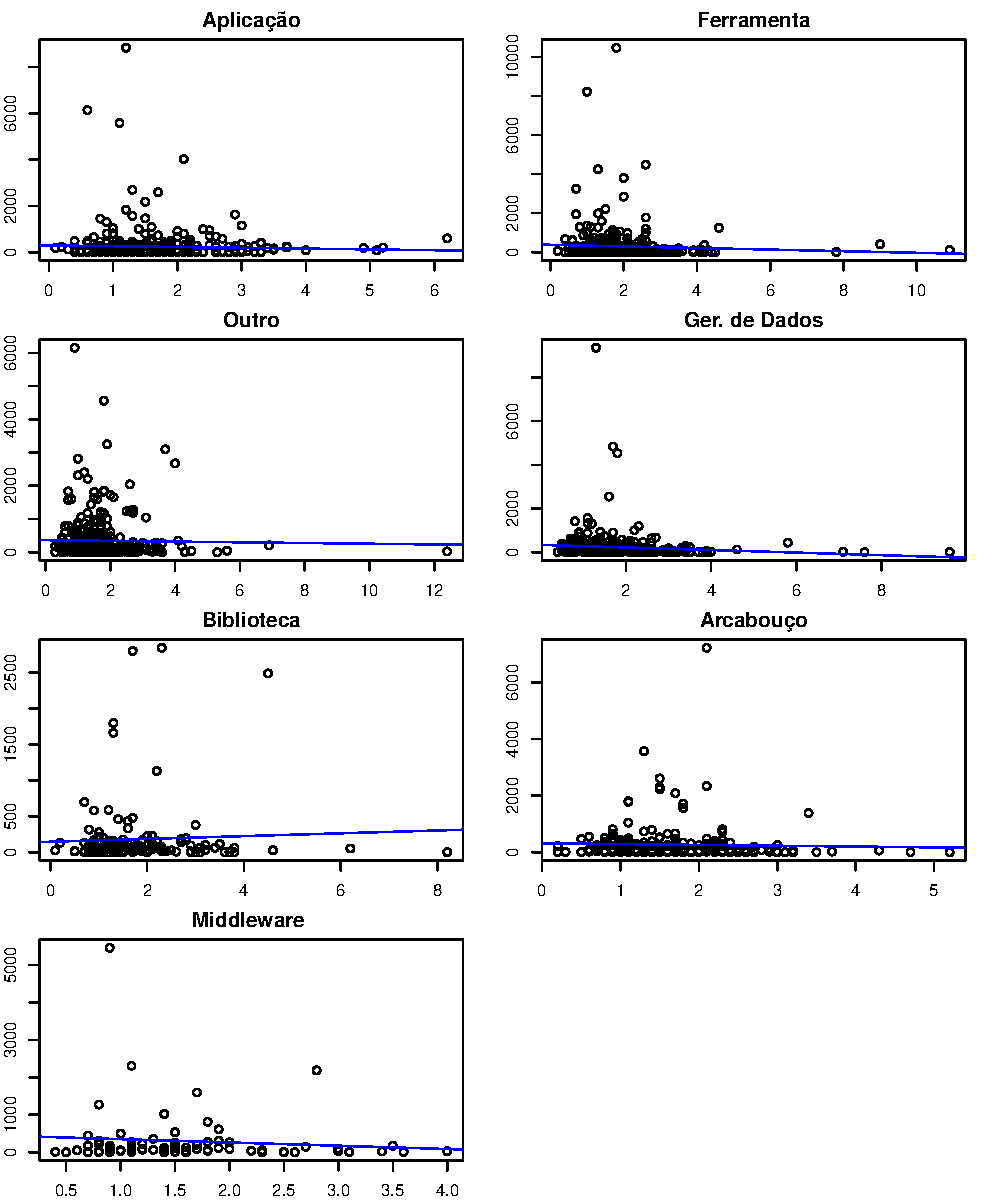
\includegraphics[trim={0cm 0cm 0cm 0cm},clip]{capitulo_estudo_caso/analise_exploratoria/correlacao_divida_pull_request.pdf}} 
  \caption{Correlação entre a dívida técnica e a quantidade de \textit{Pull requests}.}
  \label{fig:correlacao_divida_pull_request} 
\end{figure}



\subsection{Colaboração}

Utilizamos três modelos diferentes para calcular a colaboração que cada um dos projetos analisados recebeu. A Tabela \ref{tab:medidas_descritivas_colaboracao} apresenta algumas medidas descritivas a respeito dos dados obtidos para os três modelos.  Já as tabelas \ref{tab:projetos_mais_colaboradores_dia}, \ref{tab:projetos_mais_colaboradores} e \ref{tab:projetos_mais_colaboracao} apresentam os projetos com maior colaboração em cada modelo de avaliação. Podemos perceber, ao analisar essas três tabelas, que há alguns projetos que figuram entre os que receberam maior colaboração, em mais de um modelo de avaliação. Esse é o caso do projeto \textit{ElasticSearch} e \textit{React-Native}.

\begin{table}[H]
\begin{tabular}{|l|l|l|l|l|l|l|}
\hline
\textbf{Modelo}           & \textbf{Min} & \textbf{1º Quart.} & \textbf{Mediana} & \textbf{Média} & \textbf{3º Quart.} & \textbf{Max} \\ \hline
Colaboradores             & 1            & 16                 & 29               & 52,7           & 56                 & 1996         \\ \hline
Colaboradores/Dias        & 108          & 16933              & 38959            & 94327          & 89801              & 3210249      \\ \hline
IC(índice de colaboração) & 5E-10        & 8,547E-07          & 2,8049E-06       & 1,08699E-05    & 8,7386E-06         & 0,000759596  \\ \hline
\end{tabular}
\caption{Medidas descritivas dos modelos de colaboração}
\label{tab:medidas_descritivas_colaboracao}
\end{table}

\subsubsection{Colaboradores/Dia}

\begin{table}[H]
\centering
\begin{tabular}{|l|l|l|}
\hline
\textbf{ID} & \textbf{URL}                                   & \textbf{Colaboradores/dias} \\ \hline
558         & https://github.com/elastic/elasticsearch       & 3210249                     \\ \hline
1773        & https://github.com/osmandapp/Osmand            & 2239425                     \\ \hline
1656        & https://github.com/apache/camel                & 2149950                     \\ \hline
523         & https://github.com/facebook/react-native       & 2067856                     \\ \hline
1713        & https://github.com/openmrs/openmrs-core        & 1806210                     \\ \hline
712         & https://github.com/swagger-api/swagger-codegen & 1503362                     \\ \hline
1838        & https://github.com/netty/netty                 & 1489200                     \\ \hline
1159        & https://github.com/pentaho/pentaho-kettle      & 1462792                     \\ \hline
1829        & https://github.com/gradle/gradle               & 1456320                     \\ \hline
1834        & https://github.com/grails/grails-core          & 1349344                     \\ \hline
\end{tabular}
\caption{Os 10 projetos com uma maior quantidade de colaboradores/dias.}
\label{tab:projetos_mais_colaboradores_dia}
\end{table}

\subsubsection{Quantidade de colaboradores}

\begin{table}[H]
\centering
\begin{tabular}{|l|l|l|}
\hline
\textbf{ID} & \textbf{URL}                                   & \textbf{Colaboradores} \\ \hline
523         & https://github.com/facebook/react-native       & 1996                   \\ \hline
558         & https://github.com/elastic/elasticsearch       & 1239                   \\ \hline
712         & https://github.com/swagger-api/swagger-codegen & 1022                   \\ \hline
936         & https://github.com/google/closure-compiler     & 858                    \\ \hline
5           & https://github.com/OpenGenus/cosmos            & 857                    \\ \hline
1325        & https://github.com/amplab/tachyon              & 819                    \\ \hline
1773        & https://github.com/osmandapp/Osmand            & 807                    \\ \hline
191         & https://github.com/openhab/openhab2-addons     & 600                    \\ \hline
1656        & https://github.com/apache/camel                & 550                    \\ \hline
1679        & https://github.com/apache/kafka                & 541                    \\ \hline
\end{tabular}
\caption{Os 10 projetos com uma maior quantidade de colaboradores}
\label{tab:projetos_mais_colaboradores}
\end{table}

\subsubsection{Assiduidade e qualidade da colaboração}

 A Tabela \ref{tab:colaboradores_maior_pagerank} apresenta os 10 colaboradores com o maior \textit{pagerank}, dentre os que contribuíram com algum dos projetos analisado.

\begin{table}[H]
\centering
\begin{tabular}{|l|l|l|}
\hline
\textbf{Login}      & \textbf{Company} & \textbf{Pagerank} \\ \hline
bitdeli-chef        & Bitdeli          & 0,002061834       \\ \hline
JakeWharton         & Square           & 0,001474745       \\ \hline
mathiasbynens       & Opera Software   & 0,000648965       \\ \hline
gaearon             & Facebook         & 0,000566109       \\ \hline
wycats              & Tilde            & 0,00049272        \\ \hline
gitter-badger       & Gitter           & 0,000491401       \\ \hline
mitsuhiko           &                  & 0,000449111       \\ \hline
orthographic-pedant &                  & 0,000417185       \\ \hline
developertown       &                  & 0,000410813       \\ \hline
tenderlove          & GitHub           & 0,000399189       \\ \hline
\end{tabular}
\caption{Os dez colaboradores com maior pagerank.}
\label{tab:colaboradores_maior_pagerank}
\end{table}


Conforme descrito anteriormente, o índice de colaboração do projeto(IC) foi medido utilizando dois aspectos de cada um dos caboladores dos projetos: qualidade e assiduidade.


\begin{table}[H]
\centering
\begin{tabular}{|l|l|l|}
\hline
\textbf{ID} & \textbf{URL}                               & \textbf{IC}          \\ \hline
51          & https://github.com/rock3r/squanchy         & 0,000759595630534000 \\ \hline
523         & https://github.com/facebook/react-native   & 0,000523447463392000 \\ \hline
5           & https://github.com/OpenGenus/cosmos        & 0,000484793043276000 \\ \hline
1839        & https://github.com/rstudio/rstudio         & 0,000312215726382000 \\ \hline
1829        & https://github.com/gradle/gradle           & 0,000260843356728000 \\ \hline
401         & https://github.com/actorapp/actor-platform & 0,000198124386547000 \\ \hline
694         & https://github.com/real-logic/Aeron        & 0,000183223347527000 \\ \hline
117         & https://github.com/treasure-data/digdag    & 0,000180137796967000 \\ \hline
1441        & https://github.com/neo4j/neo4j             & 0,000176683446184000 \\ \hline
997         & https://github.com/crate/crate             & 0,000172710067404000 \\ \hline
\end{tabular}
\caption{Os 10 projetos com o maior índice de colaboração(IC).}
\label{tab:projetos_mais_colaboracao}
\end{table}


\subsection{Produtividade}



 A Tabela \ref{tab:resultado_regressao_modelos_colaboracao} apresenta os coeficientes de cada um dos modelos de regressão e o índice de determinação $R^2$\cite{degroot2012probability}. 
 

 


\begin{table}[H]
\centering
\footnotesize
\begin{tabular}{|l|l|l|l|l|l|}
\hline
\textbf{Modelo}           & \textbf{Intercepção} & \textbf{NLOC\_5} & \textbf{WATCHERS} & \textbf{PULL\_REQUESTS} & \textbf{R2} \\ \hline
Colaboradores             & 20,4981              & 0,0001           & 0,0198            & 0,0472                  & 0,5515      \\ \hline
Colaboradores/Dia         & 27579,6746           & 0,2641           & 24,9512           & 111,2109                & 0,4347      \\ \hline
IC(índice de colaboração) & 5,65E-06             & -3,99E-12        & 5,88E-09          & 9,78E-09                & 0,2400      \\ \hline
\end{tabular}
\caption{Coeficientes angular  e coeficiente de determinação dos modelos de regressão usados para o cálculo da produtividades do projetos.}
\label{tab:resultado_regressao_modelos_colaboracao}
\end{table}


Como uma tentativa para melhorar os modelos obtidos, foi utilizado o método de seleção de modelos AIC(\textit{Akaike information criterion})\cite{sakamoto1986akaike} para verificar se algumas das variáveis independentes poderiam ser suprimidas. Entretanto, em nenhum dos três casos isso ocorreu.

As Tabelas \ref{tab:10_mais_produtivos_quantidade}, \ref{tab:10_mais_produtivos_ic} e \ref{tab:10_mais_produtivos_colaboradores_dia} apresentam os projetos mais produtividos de acordo com cada modelo de colaboração utilizado. 



\begin{table}[H]
\centering
\footnotesize
\begin{tabular}{|l|l|l|l|l|}
\hline
\textbf{ID} & \textbf{URL}                                             & \textbf{Colab.} & \textbf{Colab. Ajus.} & \textbf{Produtividade} \\ \hline
392         & https://github.com/takayanagi2087/dataforms              & 1                & 22,88                & 22,88                    \\ \hline
728         & https://github.com/peter-mount/opendata                  & 2                & 24,93                & 12,46                   \\ \hline
1425        & https://github.com/cderoove/damp.ekeko.snippets          & 6                & 72,29                & 12,04                    \\ \hline
187         & https://github.com/metasfresh/metasfresh                 & 23               & 206,38                & 8,97                    \\ \hline
586         & https://github.com/jflex-de/jflex                        & 9                & 71,68                & 7,96                   \\ \hline
633         & https://github.com/Subterranean-Security/Crimson         & 3                & 23,82                & 7,94                    \\ \hline
628         & https://github.com/google/FreeBuilder                    & 6                & 46,69                & 7,78                    \\ \hline
1091        & https://github.com/SurvivalGamesDevTeam/TheSurvivalGames & 3                & 22,95                & 7,65                    \\ \hline
107         & https://github.com/sroy9/equation-parsing                & 3                & 20,95                & 6,98                    \\ \hline
155         & https://github.com/NumberFour/n4js                       & 19               & 131,77                & 6,93                    \\ \hline
\end{tabular}
\caption{Os 10 projetos mais produtivos de acordo com o modelo de colaboração de quantidade.}
\label{tab:10_mais_produtivos_quantidade}
\end{table}


\begin{table}[H]
\centering
\footnotesize
\begin{tabular}{|l|l|l|l|l|}
\hline
\textbf{ID} & \textbf{URL}                                & \textbf{IC} & \textbf{IC Ajus.} & \textbf{Produtividade} \\ \hline
563         & https://github.com/clc/eyes-free            & 4,80E-10    & 5,21E-06          & 10867,44               \\ \hline
549         & https://github.com/esnet/oscars             & 5,43E-10    & 5,40E-06          & 9946,88                \\ \hline
376         & https://github.com/WorldGrower/WorldGrower  & 7,87E-10    & 5,33E-06          & 6771,79                \\ \hline
392         & https://github.com/takayanagi2087/dataforms & 8,33E-10    & 5,60E-06          & 6718,67                \\ \hline
497         & https://github.com/ekiwi/jade-mirror        & 1,25E-09    & 5,17E-06          & 4136,80                \\ \hline
124         & https://github.com/software-jessies-org/scm & 1,54E-09    & 5,64E-06          & 3651,52                \\ \hline
891         & https://github.com/walkingthumbs/smack      & 2,09E-09    & 5,41E-06          & 2587,62                \\ \hline
688         & https://github.com/scottbell/biosim         & 2,30E-09    & 4,06E-06          & 1762,86                \\ \hline
770         & https://github.com/kuali-mirror/kpme        & 3,58E-09    & 5,08E-06          & 1418,17                \\ \hline
217         & https://github.com/byu-vv-lab/civl          & 4,74E-09    & 5,41E-06          & 1140,24                \\ \hline
\end{tabular}
\caption{Os 10 projetos mais produtivos de acordo com o modelo de colaboração de assiduidade e qualidade (IC).}
\label{tab:10_mais_produtivos_ic}
\end{table}

\begin{table}[H]
\centering
\footnotesize
\begin{tabular}{|l|l|l|l|l|}
\hline
\textbf{ID} & \textbf{URL}                                                  & \textbf{C/D} & \textbf{C/D Ajus.} & \textbf{Produtividade} \\ \hline
501         & https://github.com/Iteration-3/Code                           & 108                 & 31830,15                  & 294,72                 \\ \hline
32          & https://github.com/TheNotoriousOOP/Iteration3                 & 196                 & 38057,48                  & 194,17                 \\ \hline
52          & https://github.com/WPI-CS3733-C17-Gamma/project-pather        & 280                 & 49622,29                  & 177,22                 \\ \hline
466         & https://github.com/tygron-virtual-humans/tygron-connect       & 399                 & 53578,22                  & 134,28                 \\ \hline
372         & https://github.com/leonnorth/Electricity                      & 224                 & 29311,97                  & 130,86                 \\ \hline
304         & https://github.com/The-Team-Awesome/Zompocalypse              & 240                 & 29340,49                  & 122,25                 \\ \hline
20          & https://github.com/ProgrammingLife2017/DynamiteAndButterflies & 378                 & 41650,63                  & 110,19                 \\ \hline
146         & https://github.com/Betta-Testers/Imbrius-Kabasuji             & 315                 & 33100,09                  & 105,08                 \\ \hline
331         & https://github.com/hungnguyen94/BTrouble                      & 354                 & 37111,68                  & 104,84                 \\ \hline
309         & https://github.com/EmperorJack/Lunarcy-Repo                   & 297                 & 29441,63                  & 99,13                  \\ \hline
\end{tabular}
\caption{Os 10 projetos mais produtivos de acordo com o modelo de colaboração de colaboradores/dia (C/D).}
\label{tab:10_mais_produtivos_colaboradores_dia}
\end{table}

Existem alguns aspectos a respeito do cálculo de produtividade que chamam a atenção. O primeiro deles é o fato de que nenhum dos projetos mais produtivos aparece entre os projetos que receberam mais colaboração. Isso é um indício de que projetos menores e com menos visibilidade conseguem ser mais produtivos do que projetos maiores e populares. Outro aspecto que chama a atenção é a elevada produtividade de alguns projetos quando ela é analisada usando o modelo de assiduidade e qualidade. Na Tabela \ref{tab:10_mais_produtivos_ic}  podemos observar que o projeto de ID 563 é o projeto mais produtivo. Esse projeto, utiliza 10867,44 vezes menos colaboração do que a esperada para produzir os resultados obtidos pelo projeto.  Claramente esse valor demasiadamente alto é uma evidência da ineficácia desse modelo. Isso se torna mais evidente quando comparamos esse resultado com o obtido nos outros modelos como o de quantidade de colaboradores. Nesse modelo, o mais produtivo é o projeto com o  ID 392. Entretanto, esse projeto utiliza 22,88 vezes menos colaboradores do que o esperado.  



\section{Análise dos juros}

 

As tabelas \ref{tab:estimacao_juros_dominio_analise} e \ref{tab:estimacao_juros_topico_analise} apresentam os resultados da estimação dos juros da dívida técnica agrupados por domínio e por tópico, respectivamente. Nessa tabela são apresentadas as produtividades médias dos projetos em cada cenário. Essa produtividade é medida utilizando os três modelos de colaboração usados neste estudo de caso. Por exemplo, observando a Tabela \ref{tab:estimacao_juros_dominio_analise}, os projetos que possuem, proporcionalmente, pouca dívida técnica, no domínio Ferramenta,  possuem uma produtividade média de 1,84. Já os projetos com um nível normal ou alto de dívida técnica, possuem uma produtividade média de 1,55 quando utilizado o modelo de produtividade 1 (Quantidade de colaboradores). Ou seja, os projetos com pouca dívida técnica têm, em média, uma produtividade 16\% maior do que os projetos com dívida técnical normal ou alta, quando essa produtividade é medida usando o modelo baseado na quantidade de colaboradores.

É possível notar, na Tabela \ref{tab:estimacao_juros_dominio_analise}, que os projetos sem dívida técnica apresentam até 38\% de produtividade média maior do que os projetos com dívida técnica. Já quando o agrupamento é feito pelos tópicos do LDA, esse número chega a 59\%.

Um resultado importante da aplicação do modelo de estimação dos juros é o fato de que em alguns casos a produtividade dos projetos com dívida técnica é maior do que a dos projetos sem dívida técnica. Isso, acontece menos nos modelos de colaboração baseados em quantidade e e colaboradores/dia. Porém, acontece, na maioria dos casos, quando o modelo de assiduidade e colaboração é utilizado. Isso é um indício forte de que esse modelo se mostra inadequado para avaliar a produtividade dos projetos. 






\begin{table}[H]
\centering
\footnotesize
\begin{tabular}{|l|l|l|l|l|l|l|l|}
\hline
\textbf{Domínio}               & \textbf{Cenário} & \pbox{3cm}{\textbf{Modelo 1}} & \textbf{Juros}         &  \pbox{3cm}{\textbf{Modelo 2}} & \textbf{Juros}          &  \pbox{3cm}{\textbf{Modelo 3}} & \textbf{Juros}          \\ \hline
\multirow{2}{*}{Biblioteca}    & Sem dívida              & 1,54            & \multirow{2}{*}{-3\%}  & 6,52            & \multirow{2}{*}{1\%}    & 2,43            & \multirow{2}{*}{-10\%}  \\ \cline{2-3} \cline{5-5} \cline{7-7}
                               & Com dívida           & 1,59            &                        & 6,47            &                         & 2,66            &                         \\ \hline
\multirow{2}{*}{Ferramenta}    & Sem dívida              & 1,84            & \multirow{2}{*}{16\%}  & 3,45            & \multirow{2}{*}{-104\%} & 4,27            & \multirow{2}{*}{27\%}   \\ \cline{2-3} \cline{5-5} \cline{7-7}
                               & Com dívida           & 1,55            &                        & 7,02            &                         & 3,13            &                         \\ \hline
\multirow{2}{*}{Outro}         & Sem dívida              & 1,96            & \multirow{2}{*}{38\%}  & 4,97            & \multirow{2}{*}{-14\%}  & 3,06            & \multirow{2}{*}{30\%}   \\ \cline{2-3} \cline{5-5} \cline{7-7}
                               & Com dívida           & 1,21            &                        & 5,69            &                         & 2,13            &                         \\ \hline
\multirow{2}{*}{Aplicação}     & Sem dívida              & 1,81            & \multirow{2}{*}{11\%}  & 5,17            & \multirow{2}{*}{-39\%}  & 3,93            & \multirow{2}{*}{11\%}   \\ \cline{2-3} \cline{5-5} \cline{7-7}
                               & Com dívida           & 1,60            &                        & 7,21            &                         & 3,49            &                         \\ \hline
\multirow{2}{*}{Arcabouço}     & Sem dívida              & 2,14            & \multirow{2}{*}{30\%}  & 8,08            & \multirow{2}{*}{22\%}   & 4,89            & \multirow{2}{*}{44\%}   \\ \cline{2-3} \cline{5-5} \cline{7-7}
                               & Com dívida           & 1,50            &                        & 6,28            &                         & 2,76            &                         \\ \hline
\multirow{2}{*}{Ger. de Dados} & Sem dívida              & 2,11            & \multirow{2}{*}{28\%}  & 8,23            & \multirow{2}{*}{4\%}    & 5,91            & \multirow{2}{*}{53\%}   \\ \cline{2-3} \cline{5-5} \cline{7-7}
                               & Com dívida           & 1,53            &                        & 7,89            &                         & 2,81            &                         \\ \hline
\multirow{2}{*}{Middleware}    & Sem dívida              & 1,27            & \multirow{2}{*}{-34\%} & 3,16            & \multirow{2}{*}{-65\%}  & 1,28            & \multirow{2}{*}{-158\%} \\ \cline{2-3} \cline{5-5} \cline{7-7}
                               & Com dívida           & 1,70            &                        & 5,23            &                         & 3,31            &                         \\ \hline
\end{tabular}
\caption{Estimação dos juros da dívida técnica por domínio utilizando os três modelos de produtividade: (1) Quantidade de colaboradores (2) Assiduidade e qualidade da colaboração (3) Colaboradores/Dia}
\label{tab:estimacao_juros_dominio_analise}
\end{table}

\small
\begin{longtable}{|l|l|l|l|l|l|l|l|l|}
\hline
\textbf{Domínio}               & \textbf{Tópico}            & \textbf{Cenário} & \textbf{Modelo 1} & \textbf{Juros}          &  \textbf{Modelo 2} & \textbf{Juros}           &  \textbf{Modelo 3} & \textbf{Juros}                   \\ \endhead \hline
\multirow{2}{*}{Aplicação}     & \multirow{2}{*}{Tópico 1}  & Sem dívida              & 1,31            & \multirow{2}{*}{-21\%}  & 1,50            & \multirow{2}{*}{-270\%}  & 7,98            & \multirow{2}{*}{59\%}   \\ \cline{3-4} \cline{6-6} \cline{8-8}
                               &                            & Com dívida           & 1,59            &                         & 5,54            &                          & 3,26            &                         \\ \hline
\multirow{2}{*}{Aplicação}     & \multirow{2}{*}{Tópico 10} & Sem dívida              & 2,34            & \multirow{2}{*}{40\%}   & 8,01            & \multirow{2}{*}{-14\%}   & 4,60            & \multirow{2}{*}{61\%}   \\ \cline{3-4} \cline{6-6} \cline{8-8}
                               &                            & Com dívida           & 1,40            &                         & 9,10            &                          & 1,79            &                         \\ \hline
\multirow{2}{*}{Outro}         & \multirow{2}{*}{Tópico 11} & Sem dívida              & 1,51            & \multirow{2}{*}{4\%}    & 1,13            & \multirow{2}{*}{-508\%}  & 1,65            & \multirow{2}{*}{-22\%}  \\ \cline{3-4} \cline{6-6} \cline{8-8}
                               &                            & Com dívida           & 1,45            &                         & 6,87            &                          & 2,01            &                         \\ \hline
\multirow{2}{*}{Ger. de Dados} & \multirow{2}{*}{Tópico 12} & Sem dívida              & 2,02            & \multirow{2}{*}{34\%}   & 8,10            & \multirow{2}{*}{0\%}     & 4,33            & \multirow{2}{*}{53\%}   \\ \cline{3-4} \cline{6-6} \cline{8-8}
                               &                            & Com dívida           & 1,32            &                         & 8,09            &                          & 2,05            &                         \\ \hline
\multirow{2}{*}{Outro}         & \multirow{2}{*}{Tópico 13} & Sem dívida              & 2,04            & \multirow{2}{*}{45\%}   & 5,53            & \multirow{2}{*}{0\%}     & 3,04            & \multirow{2}{*}{33\%}   \\ \cline{3-4} \cline{6-6} \cline{8-8}
                               &                            & Com dívida           & 1,13            &                         & 5,53            &                          & 2,05            &                         \\ \hline
\multirow{2}{*}{Middleware}    & \multirow{2}{*}{Tópico 14} & Sem dívida              & 1,81            & \multirow{2}{*}{3\%}    & 1,93            & \multirow{2}{*}{-234\%}  & 1,23            & \multirow{2}{*}{-157\%} \\ \cline{3-4} \cline{6-6} \cline{8-8}
                               &                            & Com dívida           & 1,75            &                         & 6,45            &                          & 3,16            &                         \\ \hline
                               

\multirow{2}{*}{Biblioteca}    & \multirow{2}{*}{Tópico 15} & Sem dívida              & 2,91            & 44\%                    & 18,83           & \multirow{2}{*}{75\%}    & 4,02            & \multirow{2}{*}{22\%}   \\ \cline{3-6} \cline{8-8}
                               &                            & Com dívida           & 1,62            &                         & 4,76            &                          & 3,16            &                         \\ \hline
\multirow{2}{*}{Biblioteca}    & \multirow{2}{*}{Tópico 16} & Sem dívida              & 1,50            & \multirow{2}{*}{0\%}    & 9,09            & \multirow{2}{*}{27\%}    & 2,28            & \multirow{2}{*}{-10\%}  \\ \cline{3-4} \cline{6-6} \cline{8-8}
                               &                            & Com dívida           & 1,51            &                         & 6,60            &                          & 2,50            &                         \\ \hline

\multirow{2}{*}{Aplicação}     & \multirow{2}{*}{Tópico 17} & Sem dívida              & 3,10            & \multirow{2}{*}{43\%}   & 3,33            & \multirow{2}{*}{-141\%}  & 4,65            & \multirow{2}{*}{-4\%}   \\ \cline{3-4} \cline{6-6} \cline{8-8}
                               &                            & Com dívida           & 1,78            &                         & 8,02            &                          & 4,82            &                         \\ \hline
\multirow{2}{*}{Arcabouço}     & \multirow{2}{*}{Tópico 18} & Sem dívida              & 2,41            & \multirow{2}{*}{22\%}   & 18,06           & \multirow{2}{*}{78\%}    & 7,55            & \multirow{2}{*}{28\%}   \\ \cline{3-4} \cline{6-6} \cline{8-8}
                               &                            & Com dívida           & 1,88            &                         & 3,96            &                          & 5,45            &                         \\ \hline
\multirow{2}{*}{Arcabouço}     & \multirow{2}{*}{Tópico 19} & Sem dívida              & 1,91            & \multirow{2}{*}{3\%}    & 0,28            & \multirow{2}{*}{-2262\%} & 1,94            & \multirow{2}{*}{-46\%}  \\ \cline{3-4} \cline{6-6} \cline{8-8}
                               &                            & Com dívida           & 1,85            &                         & 6,64            &                          & 2,83            &                         \\ \hline
\multirow{2}{*}{Ger. de Dados} & \multirow{2}{*}{Tópico 2}  & Sem dívida              & 2,58            & \multirow{2}{*}{38\%}   & 4,09            & \multirow{2}{*}{-43\%}   & 3,47            & \multirow{2}{*}{28\%}   \\ \cline{3-4} \cline{6-6} \cline{8-8}
                               &                            & Com dívida           & 1,59            &                         & 5,84            &                          & 2,51            &                         \\ \hline
\multirow{2}{*}{Arcabouço}     & \multirow{2}{*}{Tópico 20} & Sem dívida              & 1,78            & \multirow{2}{*}{1\%}    & 2,61            & \multirow{2}{*}{-274\%}  & 2,52            & \multirow{2}{*}{-43\%}  \\ \cline{3-4} \cline{6-6} \cline{8-8}
                               &                            & Com dívida           & 1,76            &                         & 9,78            &                          & 3,60            &                         \\ \hline
\multirow{2}{*}{Ger. de Dados} & \multirow{2}{*}{Tópico 21} & Sem dívida              & 2,01            & \multirow{2}{*}{19\%}   & 12,21           & \multirow{2}{*}{29\%}    & 5,61            & \multirow{2}{*}{40\%}   \\ \cline{3-4} \cline{6-6} \cline{8-8}
                               &                            & Com dívida           & 1,63            &                         & 8,69            &                          & 3,34            &                         \\ \hline
\multirow{2}{*}{Aplicação}     & \multirow{2}{*}{Tópico 22} & Sem dívida              & 1,81            & \multirow{2}{*}{18\%}   & 1,54            & \multirow{2}{*}{-154\%}  & 8,59            & \multirow{2}{*}{51\%}   \\ \cline{3-4} \cline{6-6} \cline{8-8}
                               &                            & Com dívida           & 1,48            &                         & 3,92            &                          & 4,23            &                         \\ \hline
\multirow{2}{*}{Ferramenta}    & \multirow{2}{*}{Tópico 23} & Sem dívida              & 1,38            & \multirow{2}{*}{-11\%}  & 2,68            & \multirow{2}{*}{-110\%}  & 4,30            & \multirow{2}{*}{32\%}   \\ \cline{3-4} \cline{6-6} \cline{8-8}
                               &                            & Com dívida           & 1,53            &                         & 5,64            &                          & 2,92            &                         \\ \hline
\multirow{2}{*}{Ger. de Dados} & \multirow{2}{*}{Tópico 24} & Sem dívida              & 2,12            & \multirow{2}{*}{26\%}   & 2,69            & \multirow{2}{*}{-276\%}  & 6,22            & \multirow{2}{*}{60\%}   \\ \cline{3-4} \cline{6-6} \cline{8-8}
                               &                            & Com dívida           & 1,57            &                         & 10,12           &                          & 2,47            &                         \\ \hline
\multirow{2}{*}{Ger. de Dados} & \multirow{2}{*}{Tópico 25} & Sem dívida              & 2,42            & \multirow{2}{*}{49\%}   & 0,69            & \multirow{2}{*}{-649\%}  & 3,80            & \multirow{2}{*}{31\%}   \\ \cline{3-4} \cline{6-6} \cline{8-8}
                               &                            & Com dívida           & 1,24            &                         & 5,14            &                          & 2,63            &                         \\ \hline
\multirow{2}{*}{Biblioteca}    & \multirow{2}{*}{Tópico 26} & Sem dívida              & 1,51            & \multirow{2}{*}{-11\%}  & 1,77            & \multirow{2}{*}{-270\%}  & 2,54            & \multirow{2}{*}{7\%}    \\ \cline{3-4} \cline{6-6} \cline{8-8}

                               &                            & Com dívida           & 1,68            &                         & 6,57            &                          & 2,37            &                         \\ \hline
                               
\newpage
\hline
\multirow{2}{*}{Arcabouço}     & \multirow{2}{*}{Tópico 27} & Sem dívida              & 1,77            & \multirow{2}{*}{37\%}   & 1,41            & \multirow{2}{*}{-89\%}   & 2,15            & \multirow{2}{*}{15\%}   \\ \cline{3-4} \cline{6-6} \cline{8-8}
                               &                            & Com dívida           & 1,12            &                         & 2,67            &                          & 1,83            &                         \\ \hline
\multirow{2}{*}{Aplicação}     & \multirow{2}{*}{Tópico 28} & Sem dívida              & 1,38            & \multirow{2}{*}{-82\%}  & 2,06            & \multirow{2}{*}{-388\%}  & 1,96            & \multirow{2}{*}{-76\%}  \\ \cline{3-4} \cline{6-6} \cline{8-8}
                               &                            & Com dívida           & 2,51            &                         & 10,05           &                          & 3,46            &                         \\ \hline
\multirow{2}{*}{Outro}         & \multirow{2}{*}{Tópico 29} & Sem dívida              & 1,73            & \multirow{2}{*}{14\%}   & 0,91            & \multirow{2}{*}{-558\%}  & 5,31            & \multirow{2}{*}{51\%}   \\ \cline{3-4}

 \cline{6-6} \cline{8-8}
                               &                            & Com dívida           & 1,49            &                         & 5,97            &                          & 2,61            &                         \\ \hline 

\multirow{2}{*}{Ferramenta}    & \multirow{2}{*}{Tópico 3}  & Sem dívida              & 1,83            & \multirow{2}{*}{13\%}   & 4,37            & \multirow{2}{*}{-116\%}  & 2,84            & \multirow{2}{*}{-23\%}  \\ \cline{3-4} \cline{6-6} \cline{8-8} 
                               &                            & Com dívida           & 1,58            &                         & 9,44            &                          & 3,49            &                         \\ \hline
                               

\multirow{2}{*}{Ferramenta}    & \multirow{2}{*}{Tópico 30} & Sem dívida              & 1,99            & \multirow{2}{*}{9\%}    & 0,28            & \multirow{2}{*}{-2454\%} & 2,84            & \multirow{2}{*}{-30\%}  \\ \cline{3-4} \cline{6-6} \cline{8-8}
                               &                            & Com dívida           & 1,81            &                         & 7,18            &                          & 3,70            &                         \\ \hline
\multirow{2}{*}{Aplicação}     & \multirow{2}{*}{Tópico 4}  & Sem dívida              & 0,66            & \multirow{2}{*}{-119\%} & 3,57            & \multirow{2}{*}{-24\%}   & 0,69            & \multirow{2}{*}{-317\%} \\ \cline{3-4} \cline{6-6} \cline{8-8}
                               &                            & Com dívida           & 1,45            &                         & 4,44            &                          & 2,89            &                         \\ \hline

\multirow{2}{*}{Ger. de Dados} & \multirow{2}{*}{Tópico 5}  & Sem dívida              & 3,57            & \multirow{2}{*}{59\%}   & 8,96            & \multirow{2}{*}{34\%}    & 14,05           & \multirow{2}{*}{79\%}   \\ \cline{3-4} \cline{6-6} \cline{8-8}
                               &                            & Com dívida           & 1,45            &                         & 5,93            &                          & 2,96            &                         \\ \hline
\multirow{2}{*}{Arcabouço}                      & \multirow{2}{*}{Tópico 6}  & Sem dívida              & 2,17            & \multirow{2}{*}{36\%}   & 11,01           & \multirow{2}{*}{34\%}    & 5,08            & \multirow{2}{*}{58\%}  \\ \cline{3-4} \cline{6-6} \cline{8-8}
                      &                            & Com dívida           & 1,40            &                         & 7,30            &                          & 2,11            &                         \\ \hline
\multirow{2}{*}{Middleware}                     & \multirow{2}{*}{Tópico 7}  & Sem dívida              & 1,17            & \multirow{2}{*}{-41\%}  & 3,40            & \multirow{2}{*}{-25\%}   & 1,27            & \multirow{2}{*}{-176\%} \\ \cline{3-4} \cline{6-6} \cline{8-8}
                     &                            & Com dívida           & 1,65            &                         & 4,25            &                          & 3,49            &                         \\ \hline
\multirow{2}{*}{Biblioteca}                     & \multirow{2}{*}{Tópico 8}  & Sem dívida              & 2,10            & \multirow{2}{*}{29\%}   & 10,01           & \multirow{2}{*}{23\%}    & 2,23            & \multirow{2}{*}{-18\%}  \\ \cline{3-4} \cline{6-6} \cline{8-8}
                     &                            & Com dívida           & 1,49            &                         & 7,69            &                          & 2,62            &                         \\ \hline
\multirow{2}{*}{Aplicação}                       & \multirow{2}{*}{Tópico 9}  & Sem dívida              & 2,12            & \multirow{2}{*}{24\%}   & 8,01            & \multirow{2}{*}{-10\%}   & 4,51            & \multirow{2}{*}{31\%}  \\ \cline{3-4} \cline{6-6} \cline{8-8}
                      &                            & Com dívida           & 1,61            &                         & 8,78            &                          & 3,13            &                         \\ \hline
\caption{Estimação dos juros da dívida técnica por tópico utilizando os três modelos de produtividade: (1) Quantidade de colaboradores (2) Assiduidade e qualidade da colaboração (3) Colaboradores/Dia}
\label{tab:estimacao_juros_topico_analise}
\end{longtable}

\normalsize

\section{Conclusões}

Neste capítulo descrevemos detalhes a respeito da execução  de cada uma das cinco etapas do estudo de caso planejado no Capítulo \ref{cap_estudo_caso}. Apresentamos os detalhes das parametrizações das ferramentas utilizadas e os resultados obtidos em cadas uma das etapas.   Um dos resultados obtidos é a estimativa de que os projetos podem ser em média até 59\% menos produtivos devido à existência da dívida técnica. 

